\documentclass[journal]{IEEEtran}
\usepackage{amsmath,amssymb}
\usepackage{booktabs,multirow,array}
\usepackage{pifont}
\usepackage{xcolor}
\usepackage{cite}
\usepackage{tikz}
\usetikzlibrary{positioning,arrows.meta}
\usepackage{algorithm}
\usepackage{algpseudocode}
\usepackage[hidelinks]{hyperref}

\newcommand{\cmark}{\ding{51}}
\newcommand{\xmark}{\ding{55}}
\newcommand{\todo}[1]{\textcolor{red}{[#1]}}
\algrenewcommand\algorithmicrequire{\textbf{Input:}}
\algrenewcommand\algorithmicensure{\textbf{Output:}}

\begin{document}

\title{AutoML-IoT: Controlled Comparison of Automated Machine Learning for IoT Anomaly Detection}
\author{\todo{Author names and affiliations}}
\maketitle

\begin{abstract}
We study how reliably automated machine learning (AutoML) selects anomaly detection models for Internet of Things (IoT) systems, and we show that the evaluation protocol influences the reported performance more than the choice of framework. We compare the widely used frameworks Auto-sklearn and H2O AutoML on public sensor and network-traffic datasets under identical data, search budgets, thread counts, and random seeds, with default models as a reference. We propose AutoML-IoT, an evaluation pipeline that audits the data, constructs leakage-aware protocols, runs controlled searches, measures detection quality and deployment cost, and explains the selected models. We provide empirical evidence that holding out entire recording blocks lowers the score of every method, whereas the difference between the frameworks stays within the variation across random seeds. We also show that duplicated and label-ambiguous records, which cover 40.5\% of the rows of a traffic dataset, bound the attainable accuracy at 0.72. We then identify the effects of class balancing, data cleaning, and split strategy on the ranking of the frameworks. Both frameworks perform close to a default random forest, but they differ substantially in model size and prediction latency. Permutation importance indicates that both frameworks rely on the same few traffic statistics. We release code and per-run results to support replication.

\end{abstract}

\begin{IEEEkeywords}
AutoML, IoT anomaly detection, Auto-sklearn, H2O AutoML, evaluation methodology, data leakage, predictive maintenance, explainability.
\end{IEEEkeywords}

\section{Introduction}\label{sec:intro}
Internet of Things (IoT) systems connect physical devices that carry sensors and network interfaces and that exchange data with remote servers~\cite{atzori2010,gubbi2013}. These systems now support agriculture, health monitoring, smart homes, and manufacturing. As deployments grow, operators must detect anomalies that indicate physical faults or cyberattacks, because undetected anomalies cause unplanned downtime, quality loss, and security incidents.

Anomalies in IoT systems originate from physical faults and from cyberattacks. A worn bearing or an unbalanced motor changes the vibration that attached sensors record, and an unnoticed fault can halt a machine without warning~\cite{wang2018,gummadi2024xaiiot}. In networks, consumer devices such as doorbells, thermostats, baby monitors, and security cameras can be infected by botnets such as Mirai and Gafgyt and then used to attack other hosts~\cite{meidan2018nbaiot,antonakakis2017}. In both cases, the observed readings or traffic deviate from normal behavior~\cite{chandola2009}.

Early detection of such anomalies supports predictive maintenance in manufacturing, since repairs can be planned before a failure occurs~\cite{wang2018}. Low-cost MEMS accelerometers cost a fraction of the price of piezoelectric sensors but sample at low rates, which yields sparse data~\cite{gummadi2024xaiiot}. In networks, signature-based detection identifies known attacks but struggles with new threats and changing attack patterns~\cite{asad2022}. Learned anomaly detectors can close part of this gap, provided that their models respect the memory and latency limits of IoT gateways.

Prior work has applied machine learning to anomaly detection in IoT sensor data and network traffic~\cite{vinayakumar2019,tama2019,bibers2024,gummadi2024xaiiot}. However, most of the existing work selects and tunes models manually, and the conclusions depend on the dataset and on the evaluation protocol. For example, a neural network performed best on sensor data in~\cite{gummadi2024xaiiot}, whereas ensemble methods performed best on botnet traffic in the same study.

Automated machine learning (AutoML) frameworks aim to remove this manual effort by searching jointly over learning algorithms and their hyperparameters~\cite{thornton2013,feurer2015,ledell2020}. Automated pipelines have also been proposed for intrusion detection~\cite{yang2024automl,injadat2021,guntur2025autoai} and for industrial IoT traffic~\cite{sezgin2023}. However, these studies address network traffic, and independent comparisons between frameworks remain rare.

On the contrary, evaluating AutoML on IoT data requires particular care. Public security datasets are known to contain labeling errors, duplicated records, and leakage between training and test partitions~\cite{engelen2021,lanvin2023,kapoor2023}. IoT datasets may share these problems, and then the reported advantage of a framework may reflect the evaluation protocol instead of the framework itself.

There are articles discussing evaluation pitfalls in security and machine learning~\cite{arp2022,kapoor2023}, none of which however examines how these pitfalls change conclusions about AutoML frameworks on IoT data. Our work bridges this gap by auditing public IoT datasets, constructing leakage-aware protocols, and comparing AutoML frameworks under identical conditions.

There are recent works~\cite{guntur2025autoai,velnambi2026} that have compared Auto-sklearn and H2O AutoML on intrusion detection data. However, these works have the following limitations that our study addresses. They address network traffic and do not consider IoT sensor data. In our earlier study~\cite{velnambi2026}, the frameworks received different training data and search budgets, so the observed differences could not be attributed to the frameworks. Moreover, neither work audits the benchmark data before it ranks the methods. The difference between AutoML-IoT and previous related work is shown in Table~\ref{tab:related}.
\begin{table*}[t]
\centering
\caption{Comparison between prior work and AutoML-IoT in terms of the available features (to our reading of the cited works).}
\label{tab:related}
\scriptsize
\setlength{\tabcolsep}{3pt}
\begin{tabular}{@{}p{1.95in}ccccccc@{}}
\toprule
System & IoT data & Automated selection & Independent comparison & Data audit & Leakage-aware protocol & Cost measured & Explanation \\
\midrule
Auto-WEKA, TPOT, Auto-sklearn, H2O AutoML, AutoGluon-Tabular \cite{thornton2013,olson2016,feurer2015,ledell2020,erickson2020} & \xmark & \cmark & \xmark & \xmark & \xmark & \xmark & \xmark \\
AMLB benchmark \cite{gijsbers2022} & \xmark & \cmark & \cmark & \xmark & \xmark & \cmark & \xmark \\
XAI-IoT \cite{gummadi2024xaiiot} & \cmark & \xmark & \xmark & \xmark & \xmark & \xmark & \cmark \\
AutoAI-IDS \cite{guntur2025autoai} & \xmark & \cmark & \cmark & \xmark & \xmark & \cmark & \xmark \\
Earlier AutoML study \cite{velnambi2026} & \xmark & \cmark & \cmark & \xmark & \xmark & \cmark & \xmark \\
CICIDS2017 audits \cite{engelen2021,lanvin2023} & \xmark & \xmark & \xmark & \cmark & \xmark & \xmark & \xmark \\
Pitfall studies \cite{arp2022,kapoor2023} & \xmark & \xmark & \xmark & \cmark & \cmark & \xmark & \xmark \\
\midrule
\textbf{AutoML-IoT (this work)} & \cmark & \cmark & \cmark & \cmark & \cmark & \cmark & \cmark \\
\bottomrule
\end{tabular}
\end{table*}


\textbf{Our contributions:} In this paper, we audit two public IoT datasets, a vibration dataset collected on a motor testbed and a traffic dataset collected from commercial devices. We then design an evaluation pipeline that we call AutoML-IoT. The pipeline consists of consecutive steps for data audit, protocol construction, controlled search, measurement, explanation, and statistical comparison, as shown in Figure~\ref{fig:pipeline}. In every step, both frameworks receive identical inputs, and default baseline models serve as a reference.
\begin{figure*}[t]
\centering
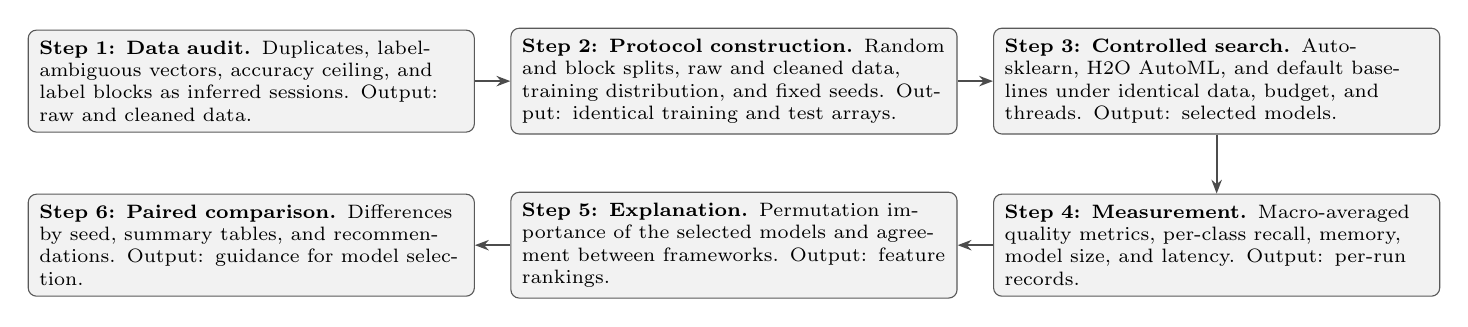
\begin{tikzpicture}[
  node distance=0.5cm and 0.45cm,
  box/.style={draw=black!65, rounded corners=3pt, fill=black!5, text width=2.12in, align=left, inner sep=4pt, font=\scriptsize},
  arr/.style={-{Stealth[length=5pt]}, thick, draw=black!70}
]
\node[box] (s1) {\textbf{Step 1: Data audit.} Duplicates, label-ambiguous vectors, accuracy ceiling, and label blocks as inferred sessions. Output: raw and cleaned data.};
\node[box, right=of s1] (s2) {\textbf{Step 2: Protocol construction.} Random and block splits, raw and cleaned data, training distribution, and fixed seeds. Output: identical training and test arrays.};
\node[box, right=of s2] (s3) {\textbf{Step 3: Controlled search.} Auto-sklearn, H2O AutoML, and default baselines under identical data, budget, and threads. Output: selected models.};
\node[box, below=0.75cm of s3] (s4) {\textbf{Step 4: Measurement.} Macro-averaged quality metrics, per-class recall, memory, model size, and latency. Output: per-run records.};
\node[box, left=of s4] (s5) {\textbf{Step 5: Explanation.} Permutation importance of the selected models and agreement between frameworks. Output: feature rankings.};
\node[box, left=of s5] (s6) {\textbf{Step 6: Paired comparison.} Differences by seed, summary tables, and recommendations. Output: guidance for model selection.};
\draw[arr] (s1) -- (s2);
\draw[arr] (s2) -- (s3);
\draw[arr] (s3) -- (s4);
\draw[arr] (s4) -- (s5);
\draw[arr] (s5) -- (s6);
\end{tikzpicture}
\caption{A high-level overview of AutoML-IoT. A labeled IoT dataset passes through six consecutive steps that produce comparable records for every method.}
\label{fig:pipeline}
\end{figure*}


We show that the evaluation protocol changes the reported performance more than the choice of framework. In particular, holding out entire recording blocks lowers the macro-averaged F1 score of all methods, whereas the differences between the frameworks stay within the variation across random seeds. We also show that label-ambiguous records bound the attainable accuracy on the traffic data and that both frameworks perform close to a default random forest. The frameworks differ mainly in the size and latency of the selected models. In obtaining these results, we address challenges that are specific to IoT data. These include the absence of session identifiers in the sensor data, repeated and conflicting records in the traffic data, and different validation strategies in the frameworks.

In summary, this paper makes the following contributions:
\begin{enumerate}
\item[(1)] We propose \emph{AutoML-IoT}, a controlled evaluation pipeline for AutoML frameworks on IoT anomaly detection. The pipeline covers data audit, leakage-aware protocol construction, controlled search, measurement of quality and cost, explanation, and paired statistical comparison.
\item[(2)] We audit a sensor dataset and a traffic dataset and quantify duplication, label ambiguity, and temporal block structure. For the traffic data, we derive an accuracy ceiling that follows from identical inputs with different labels.
\item[(3)] We compare Auto-sklearn and H2O AutoML under identical data, budgets, thread counts, and seeds, and we add default baseline models. We analyze split strategy, data cleaning, and class balancing as separate factors.
\item[(4)] We report macro-averaged quality metrics, per-class recall, selected models, memory, model size, and prediction latency for both frameworks in complete tables.
\item[(5)] We explain the selected models with permutation importance and relate the result to hand-built models from earlier work.
\item[(6)] We derive recommendations for evaluating AutoML on IoT data, and we release code and per-run results.
\end{enumerate}

\section{Background and Problem Setup}\label{sec:background}
We begin by presenting a formal model of the comparison problem, which establishes a basis that applies to any labeled IoT dataset and any AutoML framework. A simple example of our setup is shown in Figure~\ref{fig:pipeline}. A dataset is audited, converted into evaluation protocols, and used to train AutoML frameworks and baseline models under identical conditions. In this section, we formalize the data, the AutoML task, the evaluation criteria, and the sources of evaluation bias.

\subsection{Data and Task Model}
Let $\mathcal{D}=\{(x_i,y_i)\}_{i=1}^{N}$ denote a labeled IoT dataset that contains $N$ samples. The vector $x_i\in\mathbb{R}^{d}$ contains features computed from sensor readings or network traffic, and $y_i\in\mathcal{C}=\{1,\dots,K\}$ is the class label. In multi-class anomaly detection, one class represents normal operation, and the remaining classes represent fault levels or attack types. Class frequencies are typically imbalanced, and some classes contain only a few distinct samples.

An evaluation protocol $\pi$ with seed $s$ partitions $\mathcal{D}$ into a training set $\mathcal{D}_{\mathrm{tr}}$ and a test set $\mathcal{D}_{\mathrm{te}}$. We consider a random protocol, which draws a stratified random partition, and a block protocol. For time-ordered recordings, consecutive samples with identical labels form blocks, and the block protocol assigns entire blocks to the test set while it keeps every class represented in both partitions. Both protocols use the same test fraction, so that differences between them do not result from the size of the test set. A training distribution $\tau$ either keeps the training set unchanged or repeats minority-class samples until every class matches the size of the majority class.

\subsection{AutoML Model}
An AutoML framework solves the combined algorithm selection and hyperparameter optimization (CASH) problem~\cite{thornton2013}. Let $\mathcal{A}$ denote a set of learning algorithms and $\Lambda_A$ the hyperparameter space of algorithm $A\in\mathcal{A}$. Given a wall-clock budget $T$, the framework returns
\begin{equation}
(A^{*},\lambda^{*}) \in \operatorname*{arg\,min}_{A\in\mathcal{A},\;\lambda\in\Lambda_A} \mathcal{L}_{\mathrm{val}}\big(A_{\lambda};\mathcal{D}_{\mathrm{tr}}\big),
\label{eq:cash}
\end{equation}
where $\mathcal{L}_{\mathrm{val}}$ is a validation loss that is estimated on $\mathcal{D}_{\mathrm{tr}}$ only. Auto-sklearn minimizes one minus the macro-averaged F1 score on a holdout split. It uses Bayesian optimization, a meta-learning warm start, and a final weighted ensemble~\cite{feurer2015}. The ensemble predicts
\begin{equation}
\hat{y}(x)=\operatorname*{arg\,max}_{c\in\mathcal{C}}\sum_{k=1}^{M} w_k\,p_k(c\mid x),
\label{eq:ensemble}
\end{equation}
where $p_k$ denotes the class probabilities of member $k$, and the weights $w_k\ge 0$ sum to one.

H2O AutoML trains a portfolio of algorithms, ranks the models on a leaderboard by cross-validated mean per-class error, and returns the leader. The leader is either a single model or a stacked ensemble, in which a metalearner combines the predictions of base models~\cite{ledell2020}. The two frameworks therefore optimize related but not identical objectives and validate differently. We document and control these differences in Section~\ref{sec:evaluation}.

\subsection{Evaluation Model}
We evaluate a model on $\mathcal{D}_{\mathrm{te}}$ with class-wise and aggregated metrics. For class $c$, the recall, the precision, and the F1 score are
\begin{equation}
\begin{aligned}
R_c&=\frac{\mathrm{TP}_c}{\mathrm{TP}_c+\mathrm{FN}_c},\qquad P_c=\frac{\mathrm{TP}_c}{\mathrm{TP}_c+\mathrm{FP}_c},\\
\mathrm{F1}_c&=\frac{2P_cR_c}{P_c+R_c}.
\end{aligned}
\label{eq:classmetrics}
\end{equation}
The macro-averaged F1 score, the balanced accuracy, and the accuracy are
\begin{equation}
\begin{aligned}
\mathrm{MF1}&=\frac{1}{K}\sum_{c=1}^{K}\mathrm{F1}_c,\qquad \mathrm{BA}=\frac{1}{K}\sum_{c=1}^{K}R_c,\\
\mathrm{ACC}&=\frac{1}{|\mathcal{D}_{\mathrm{te}}|}\sum_{i\in\mathcal{D}_{\mathrm{te}}}\mathbb{1}[\hat{y}_i=y_i].
\end{aligned}
\label{eq:aggmetrics}
\end{equation}
Macro-averaging gives every class the same weight, so that failures on rare classes remain visible, whereas the accuracy is dominated by frequent classes. We also report the macro-averaged precision and recall, the support-weighted F1 score, and the Matthews correlation coefficient (MCC)~\cite{chicco2020}.

Because the seed $s$ fixes the split, methods are compared by paired differences. For a metric $M_s$ and two methods $m_1$ and $m_2$, we define
\begin{equation}
\begin{aligned}
\Delta_s(m_1,m_2)&=M_s(m_1)-M_s(m_2),\\
W(m_1,m_2)&=\sum_{s\in\mathcal{S}}\mathbb{1}[\Delta_s>0],
\end{aligned}
\label{eq:paired}
\end{equation}
where $\mathcal{S}$ is the set of seeds and $W$ counts the seeds in which $m_1$ wins. Cost is measured by the wall-clock fit time, the peak memory of all processes, the size of the serialized model, and the batch prediction latency per sample.

\subsection{Sources of Evaluation Bias}
Three properties of IoT datasets can distort the comparison of frameworks. The first property is the duplication and ambiguity of records. Let $n_{v,c}$ denote the number of rows with feature vector $v$ and label $c$. A vector $v$ is \emph{ambiguous} if $n_{v,c}>0$ for at least two classes. Any classifier that maps identical inputs to identical outputs assigns a single label to $v$, and therefore the accuracy on the file cannot exceed
\begin{equation}
A_{\max}=\frac{1}{N}\sum_{v}\max_{c}\,n_{v,c}.
\label{eq:ceiling}
\end{equation}
The corresponding per-class ceiling $R^{\max}_c$ is the share of class $c$ that a majority-label rule classifies correctly. Exact duplicates additionally allow identical rows to appear in the training and the test partition, which inflates the score.

The second property is temporal structure, because a random protocol can place neighboring samples of the same recording in both partitions, so that test samples have close neighbors in the training data. The third property is class imbalance, which makes the accuracy uninformative about rare classes. We quantify these properties in Section~\ref{sec:audit} and measure their effect in Section~\ref{sec:evaluation}.

\section{Data Audit Study}\label{sec:audit}
To validate the existence of evaluation bias in public IoT datasets (captured by the model in Section~\ref{sec:background}), we audited two datasets that were released for IoT anomaly detection~\cite{gummadi2024xaiiot}. The audit uses the released files without modification, and the dataset statistics are presented in Table~\ref{tab:audit}.

\subsection{MEMS Vibration Dataset}
The MEMS dataset was collected on a motor testbed with a balancing disk~\cite{gummadi2024xaiiot,abdallah2023sensors}. MEMS accelerometers record the acceleration along three axes at a sampling rate of 10\,Hz. The motor operates at ten rotational speeds between 100 and 600 revolutions per minute, and a mass mounted on the disk creates mechanical imbalance and thereby three health conditions, namely normal operation, near-failure, and failure. The released file contains 21,576 samples with three features and three classes, and it contains no session or speed column. The file encodes the conditions as the integer labels 1, 2, and 3, which contain 10,965, 5,773, and 4,838 samples. Following the class designation of~\cite{gummadi2024xaiiot}, we read these labels as normal, near-failure, and failure. MEMS accelerometers cost about \$8, compared with about \$1305 for piezoelectric sensors, but they offer lower sampling rates~\cite{gummadi2024xaiiot}.

We therefore cut the file into contiguous blocks of identical labels. This yields 15 blocks with a median length of 1,423 rows, which we use as an inferred grouping for block protocols. The z-axis shows a lag-1 autocorrelation of 0.38, whereas the x- and y-axes show 0.06 and 0.12, so that neighboring samples are partly redundant.

\subsection{N-BaIoT Traffic Dataset}
N-BaIoT contains traffic of nine commercial IoT devices, among them doorbells, a thermostat, a baby monitor, and security cameras, that were infected with the Mirai and Gafgyt botnets~\cite{meidan2018nbaiot,antonakakis2017}. The repository that accompanies~\cite{gummadi2024xaiiot} provides a subset of 20 features for each device. Each device has either six or eleven classes of equal nominal size. We audit all nine devices and use device 9, which has eleven classes and 209,000 rows, for the experiments.

Table~\ref{tab:audit} lists the audit results, in which cleaning removes exact duplicates and the rows of ambiguous vectors, so that every N-BaIoT device loses 41.8 to 48.3\% of its rows. The smallest class keeps only 9 to 23 unique rows, and two or three classes fall below 50 unique rows. MEMS, in contrast, is almost free of duplicates (0.1\%) and retains 4,832 unique rows in its smallest class.
\begin{table*}[t]
\centering
\caption{Audit of the released datasets. Bold: best N-BaIoT value per column. Smallest class: unique rows of the smallest class after cleaning.}
\label{tab:audit}
\scriptsize
\setlength{\tabcolsep}{3pt}
\begin{tabular}{@{}lrrrrrrrr@{}}
\toprule
Dataset & Classes & Rows & Unique rows & Removed (\%) & Smallest class & Ambiguous vectors & Rows in them (\%) & Accuracy ceiling \\
\midrule
mems & 3 & 21,576 & 21,551 & 0.1 & 4,832 & 6 & 0.1 & 1.000 \\
\midrule
nbaiot:1 & 11 & 220,000 & 116,635 & 47.0 & 17 & \textbf{5} & 43.4 & 0.689 \\
nbaiot:2 & 11 & 132,000 & 76,786 & \textbf{41.8} & 11 & 6 & 40.3 & 0.719 \\
nbaiot:3 & 6 & 120,000 & 68,937 & 42.6 & \textbf{23} & \textbf{5} & \textbf{39.1} & \textbf{0.833} \\
nbaiot:4 & 11 & 220,000 & 123,680 & 43.8 & 12 & 8 & 43.3 & 0.689 \\
nbaiot:5 & 11 & 220,000 & 113,767 & 48.3 & 22 & 6 & 47.4 & 0.648 \\
nbaiot:6 & 11 & 220,000 & 114,335 & 48.0 & 14 & 7 & 47.0 & 0.652 \\
nbaiot:7 & 6 & 120,000 & 66,652 & 44.5 & 19 & 7 & 39.3 & \textbf{0.833} \\
nbaiot:8 & 11 & 220,000 & 127,915 & 41.9 & 17 & 10 & 39.9 & 0.724 \\
nbaiot:9 & 11 & 209,000 & 117,073 & 44.0 & 9 & 11 & 40.5 & 0.718 \\
\bottomrule
\end{tabular}
\end{table*}


The ambiguity is more severe than the duplication of records in these datasets. On each device, 5 to 11 feature vectors occur under more than one label, and they cover 39.1 to 47.4\% of all rows. On device 9, 11 vectors cover 40.5\% of the rows. These vectors account for 99.5, 100, and 99.9\% of the rows of classes 1, 3, and 4, respectively, and a single vector occurs under eight labels (Table~\ref{tab:ambclass} in Appendix~\ref{app:audit}). Equation~\eqref{eq:ceiling} then bounds the accuracy at 0.718 on device 9 and between 0.648 and 0.833 across all devices. For MEMS, only 0.1\% of the rows are ambiguous, and the bound equals 1.000.

\textbf{Generalizability of the study:} The audit covers one sensor dataset and all nine devices of the traffic dataset. The duplication and ambiguity statistics are similar across devices, which suggests that they are a property of the released 20-feature subset and not of device 9. Random forests and ensembles reach accuracies between 0.64 and 0.83 on the same files in~\cite{gummadi2024xaiiot}, which coincides with the bounds above. We therefore hypothesize that the lower accuracy of the 20-feature subset, in comparison with all 115 features, reflects information that the subset discards and not a limited quality of the models. We could not test this hypothesis, because the full feature set is not part of the released files.

\section{Effect of Evaluation Bias on Reported Performance}\label{sec:effect}
In this section, we provide two simple examples that illustrate how label ambiguity and temporal structure change the reported performance, and we provide intuition on why evaluation protocols differ in difficulty.

\subsection{Label Ambiguity}
Consider a feature vector $v$ that occurs 60 times with label $a$ and 40 times with label $b$ in a test set. A classifier assigns a single label to $v$, and therefore it classifies at most 60 of these 100 samples correctly. The contribution of $v$ to the accuracy is bounded by 0.6, independent of the learning algorithm and of the search effort. If such vectors cover a substantial share of the file, as in the traffic data, the same bound applies to the overall score.

On the raw data of device 9, the bound of Equation~\eqref{eq:ceiling} is 0.718. The best method reaches 0.711 (Section~\ref{sec:evaluation}), which is 99\% of the bound. In this regime, a ranking of frameworks reflects tie-breaking between labels of ambiguous vectors and not the ability to detect anomalies.

\textbf{Interpretation:} Ambiguity changes the meaning of a score, because the achievable accuracy depends on the file and not on the classifier. A high accuracy on a file with ambiguous vectors indicates that the classifier learned the majority labels, and a low accuracy does not necessarily indicate a classifier of low quality. Duplicated records enlarge this effect, because the majority label of an ambiguous vector is then repeated in both partitions.

\subsection{Temporal Structure}
Consider a recording that is divided into blocks of consecutive samples. Under a random protocol, a test sample at time $t$ has training neighbors at $t-1$ and $t+1$. If neighboring measurements are similar, a classifier can interpolate between neighbors and achieves a high score without learning the boundaries between operating conditions. Under a block protocol, the neighbors of a test block are absent from the training set, and the classifier must generalize to operating conditions that it has not observed.

A preliminary probe on MEMS illustrates the size of this effect for a single learning algorithm. A random forest with 100 trees and a maximum depth of 10 reaches an accuracy of 0.71 and a macro-F1 of 0.66 under a random 70/30 split. When whole blocks are held out in five-fold validation, the values fall to $0.54\pm0.12$ and $0.35\pm0.10$.

\textbf{Interpretation:} Both effects inflate the reported performance independent of the framework. A comparison of frameworks is therefore meaningful only after the protocol has been audited and fixed. We implement this requirement in the pipeline of the next section.

\section{The AutoML-IoT Pipeline}\label{sec:pipeline}
Figure~\ref{fig:pipeline} shows the flow of AutoML-IoT, and the following subsections describe each step. The pipeline consists of six consecutive steps, and every step consumes the artifacts of the previous step. All steps use fixed seeds, so that every run is reproducible up to the nondeterminism of searches that stop on a wall-clock limit. We describe the steps in this section and evaluate them in Section~\ref{sec:evaluation}.

\subsection{Step 1: Data Audit and Cleaning}
The audit computes the unique feature vectors of a dataset and the counts $n_{v,c}$. It derives the set of ambiguous vectors, the accuracy ceiling of Equation~\eqref{eq:ceiling}, and, for time-ordered data, the contiguous blocks of identical labels. Cleaning removes exact duplicates and the rows of ambiguous vectors and thereby produces a cleaned variant of the data. The raw variant is retained, because earlier studies used it and because it allows us to measure the effect of cleaning, as summarized in Algorithm~\ref{alg:audit}.

\begin{algorithm}[t]
\caption{Data Audit and Cleaning}
\label{alg:audit}
\footnotesize
\begin{algorithmic}[1]
\Require Labeled dataset $\mathcal{D}=\{(x_i,y_i)\}_{i=1}^{N}$
\Ensure $\mathcal{D}_{\mathrm{raw}}$, $\mathcal{D}_{\mathrm{clean}}$, ceiling $A_{\max}$, blocks $g$
\State Compute the unique vectors $V$ and the counts $n_{v,c}$
\State $V_{\mathrm{amb}}\leftarrow\{v\in V:\ |\{c: n_{v,c}>0\}|\ge 2\}$
\State $A_{\max}\leftarrow \frac{1}{N}\sum_{v}\max_{c} n_{v,c}$
\State $\mathcal{D}_{\mathrm{dup}}\leftarrow$ $\mathcal{D}$ without exact duplicate rows
\State $\mathcal{D}_{\mathrm{clean}}\leftarrow$ $\mathcal{D}_{\mathrm{dup}}$ without rows whose vector is in $V_{\mathrm{amb}}$
\If{$\mathcal{D}$ is time ordered}
  \State $g(i)\leftarrow$ index of the run of identical labels that contains row $i$
\EndIf
\State \Return $\mathcal{D}$, $\mathcal{D}_{\mathrm{clean}}$, $A_{\max}$, $g$
\end{algorithmic}
\end{algorithm}

\subsection{Step 2: Protocol Construction}
For each dataset variant, this step creates the protocols of Section~\ref{sec:background} with a fixed seed. For time-ordered data, the block protocol holds out about 30\% of the blocks of every class, so that every class remains present in both partitions. The training distribution is either unchanged or oversampled to the size of the majority class. All frameworks and baselines receive identical training and test arrays, which removes differences in data handling as a confounding factor.

\subsection{Step 3: Controlled Search}
Auto-sklearn and H2O AutoML run with an identical wall-clock budget, an identical number of threads, and the same seed. Settings that cannot be equalized, namely the optimization objective and the validation strategy, are documented and reported (Table~\ref{tab:config}). Default baselines are trained on the same arrays without a search, and Algorithm~\ref{alg:run} summarizes the control flow.

\begin{algorithm}[t]
\caption{Controlled Comparison}
\label{alg:run}
\footnotesize
\begin{algorithmic}[1]
\Require Variants $\{\mathcal{D}_{\mathrm{raw}},\mathcal{D}_{\mathrm{clean}}\}$, protocols $\Pi$, distributions $\mathcal{T}$, frameworks $\mathcal{F}$, baselines $\mathcal{B}$, seeds $\mathcal{S}$, budget $T_{\max}$, threads $p$
\Ensure Records $\mathcal{R}$
\State $\mathcal{R}\leftarrow\emptyset$
\For{each variant $\mathcal{D}'$, protocol $\pi\in\Pi$, distribution $\tau\in\mathcal{T}$, seed $s\in\mathcal{S}$}
  \State $(\mathcal{D}_{\mathrm{tr}},\mathcal{D}_{\mathrm{te}})\leftarrow \textsc{Split}(\mathcal{D}',\pi,s)$
  \State $\mathcal{D}_{\mathrm{tr}}\leftarrow \textsc{Distribute}(\mathcal{D}_{\mathrm{tr}},\tau,s)$
  \For{each framework $f\in\mathcal{F}$}
    \State $m_f\leftarrow \textsc{Search}(f,\mathcal{D}_{\mathrm{tr}},T_{\max},p,s)$
  \EndFor
  \For{each baseline $b\in\mathcal{B}$}
    \State $m_b\leftarrow \textsc{Fit}(b,\mathcal{D}_{\mathrm{tr}},s)$
  \EndFor
  \For{each model $m\in\{m_f\}\cup\{m_b\}$}
    \State Append quality, per-class recall, and cost of $m$ on $\mathcal{D}_{\mathrm{te}}$ to $\mathcal{R}$
  \EndFor
  \State Compute permutation importance of $m_f$ for each $f\in\mathcal{F}$ if requested
\EndFor
\State \Return $\mathcal{R}$
\end{algorithmic}
\end{algorithm}

\subsection{Step 4: Measurement}
Every model is evaluated with the metrics of Section~\ref{sec:background}, and we take the cost measurements as follows. The fit time is the wall-clock time of the search, including the start-up of the framework. The peak memory is the maximum, over samples taken every 0.5\,s, of the summed resident set sizes of the process and all its children. This sum includes the Java process of H2O AutoML and the worker processes of Auto-sklearn. The model size is the size of the serialized model on disk. The latency is the time that a batch of up to 5,000 test samples needs for prediction, divided by the batch size, and it includes the overhead of the framework.

\subsection{Step 5: Explanation}
We explain the selected models by permutation importance~\cite{altmann2010}. For a feature $j$, the importance is the drop of the macro-averaged F1 score when the values of $j$ are shuffled,
\begin{equation}
I_j=\mathrm{MF1}(\mathcal{D}_{\mathrm{te}})-\frac{1}{R}\sum_{r=1}^{R}\mathrm{MF1}\big(\mathcal{D}^{(j,r)}_{\mathrm{te}}\big),
\label{eq:pfi}
\end{equation}
where $\mathcal{D}^{(j,r)}_{\mathrm{te}}$ is the test set with feature $j$ shuffled in repetition $r$. We use a random subset of 3,000 test rows and $R=3$ repetitions. To compare frameworks, we compute the Spearman rank correlation of the importance vectors, the overlap of the leading features, and the stability across seeds. Because correlated features can distort permutation importance~\cite{strobl2008}, we interpret the leading features and do not interpret the exact order of features with near-zero importance.

\subsection{Step 6: Paired Comparison and Reporting}
Methods are compared by the paired differences of Equation~\eqref{eq:paired} and the number of seeds won. Tables report the mean and the sample standard deviation over five seeds, and bold type marks the best value of a column. With five seeds, the smallest attainable two-sided Wilcoxon $p$-value is 0.0625. We therefore report effect sizes and win counts and declare no difference significant.

\section{Evaluation}\label{sec:evaluation}
Our evaluation of AutoML-IoT aims to answer the following questions:
\begin{itemize}
\item \textbf{RQ1:} Do AutoML models outperform default baselines once leakage is controlled?
\item \textbf{RQ2:} Does the ranking of the two frameworks survive changes of split, data cleaning, and class balancing?
\item \textbf{RQ3:} Which classes fail, and how far do accuracy and macro-F1 diverge?
\item \textbf{RQ4:} What do the frameworks cost in time, memory, model size, and latency?
\item \textbf{RQ5:} Do the selected models rely on the same features, and on those found for hand-built models~\cite{gummadi2024xaiiot}?
\end{itemize}

\subsection{Experimental Setup}
\textbf{Dataset description:} We evaluate five setups. On MEMS, we use a random stratified 70/30 split, a block split that holds out about 30\% of the blocks of each class, and the block split with an oversampled training set. On N-BaIoT device 9, we use the deduplicated variant and the raw variant, each with a random stratified 70/30 split. The random split is comparable to the protocol of~\cite{gummadi2024xaiiot}. Every setup is repeated with seeds 0 to 4, and the seed also determines the split.

\textbf{AutoML configuration:} Table~\ref{tab:config} lists the settings of both frameworks. They share the budget of 1800\,s, eight threads, and the seeds, and they differ in the objective and in the validation strategy because these settings are native to each framework. In addition, we run H2O AutoML with its \texttt{balance\_classes} option on the MEMS block split to separate algorithmic balancing from data-level oversampling, which yields 55 AutoML runs in total.

\textbf{Baselines:} The baselines are a majority-class predictor, a decision tree, a random forest with 100 trees, and an MLP, all with default settings, and the MLP uses standardized inputs. This yields 100 baseline runs, and all 155 runs share one hardware and software environment (Appendix~\ref{app:config}).
\begin{table}[t]
\centering
\caption{Configuration of the two frameworks. Both frameworks use the same budget, thread count, and seeds.}
\label{tab:config}
\scriptsize
\setlength{\tabcolsep}{3pt}
\begin{tabular}{@{}p{0.85in}p{1.2in}p{1.25in}@{}}
\toprule
Setting & Auto-sklearn & H2O AutoML \\
\midrule
Version & 0.15.0 & 3.46.0.12 \\
Objective & Macro-F1 & Mean per-class error (leaderboard) \\
Validation & Holdout, 67/33 & Cross-validation, five folds \\
Ensemble & Up to 50 models & Stacked ensembles \\
Budget & 1800\,s & 1800\,s \\
Per-configuration limit & 120\,s & Not set \\
Memory & 3072\,MB per run & 4\,GB heap \\
Threads & 8 & 8 \\
Seeds & 0 to 4 & 0 to 4 \\
\bottomrule
\end{tabular}
\end{table}


\subsection{Detection Quality on MEMS}
Table~\ref{tab:mems} reports the macro-F1 of all methods on MEMS under the three protocols, and Appendix~\ref{app:results} gives complete metrics for both frameworks. The majority-class row shows the score of a model that ignores its input. Table~\ref{tab:paired} compares the methods by paired differences.

\textbf{1) Random split:} Both frameworks outperform the default random forest in all five seeds, by 0.035 (Auto-sklearn) and 0.022 (H2O AutoML). Auto-sklearn also exceeds H2O AutoML by 0.013 in all five seeds. A default MLP stays close, with a gap of 0.018 to Auto-sklearn and 0.004 to H2O AutoML.

\textbf{2) Block split:} Holding out entire blocks lowers the macro-F1 of every learning method by 0.09 to 0.13. Auto-sklearn drops from 0.689 to 0.562 and H2O AutoML from 0.675 to 0.566. The random forest drops from 0.654 to 0.547, the MLP from 0.671 to 0.556, and the decision tree from 0.592 to 0.502.

The standard deviation over seeds grows from at most 0.007 to between 0.05 and 0.07 (0.02 for the decision tree). The scores of different methods also move together across seeds, with correlation coefficients between 0.93 and 0.99. The held-out blocks therefore explain more of the variation than the method does. Under this protocol, the two frameworks cannot be distinguished (difference $-0.004$, three seeds won and two lost). Both exceed the random forest by only 0.015 to 0.019 and the MLP by 0.006 to 0.010.

\textbf{3) Class level:} The failure class (class 3) is the most difficult class. Its recall is 0.40 for Auto-sklearn and 0.36 for H2O AutoML, with standard deviations of 0.23 and 0.22 over the seeds. The normal class (class 1) reaches 0.64 to 0.67, and the near-failure class (class 2) reaches 0.74 to 0.75 (Table~\ref{tab:perclassmems}).
\begin{table*}[t]
\centering
\caption{MEMS: mean $\pm$ standard deviation over five seeds for three protocols. Bold: highest mean per column.}
\label{tab:mems}
\scriptsize
\setlength{\tabcolsep}{3pt}
\begin{tabular}{@{}lrrrr@{}}
\toprule
Method & Macro-F1, random split & Macro-F1, block split & Macro-F1, block + oversampling & Balanced accuracy, block split \\
\midrule
Auto-sklearn & \textbf{0.689 $\pm$ 0.005} & 0.562 $\pm$ 0.063 & 0.545 $\pm$ 0.044 & \textbf{0.593 $\pm$ 0.067} \\
H2O AutoML & 0.675 $\pm$ 0.003 & \textbf{0.566 $\pm$ 0.068} & 0.540 $\pm$ 0.047 & \textbf{0.593 $\pm$ 0.075} \\
H2O AutoML, balanced & -- & 0.533 $\pm$ 0.087 & -- & 0.589 $\pm$ 0.070 \\
Random forest & 0.654 $\pm$ 0.004 & 0.547 $\pm$ 0.053 & 0.538 $\pm$ 0.040 & 0.579 $\pm$ 0.064 \\
MLP & 0.671 $\pm$ 0.007 & 0.556 $\pm$ 0.060 & \textbf{0.558 $\pm$ 0.063} & 0.586 $\pm$ 0.067 \\
Decision tree & 0.592 $\pm$ 0.007 & 0.502 $\pm$ 0.022 & 0.498 $\pm$ 0.025 & 0.539 $\pm$ 0.042 \\
Majority class & 0.225 $\pm$ 0.000 & 0.245 $\pm$ 0.014 & 0.245 $\pm$ 0.014 & 0.333 $\pm$ 0.000 \\
\bottomrule
\end{tabular}
\end{table*}

\begin{table*}[t]
\centering
\caption{Paired macro-F1 differences (first minus second method; seeds won/lost in parentheses). A: Auto-sklearn, H: H2O AutoML, DT: decision tree. Bold: first method won all five seeds.}
\label{tab:paired}
\scriptsize
\setlength{\tabcolsep}{3pt}
\begin{tabular}{@{}lrrrrrrr@{}}
\toprule
Setup & A$-$H & A$-$RF & H$-$RF & A$-$MLP & H$-$MLP & A$-$DT & H$-$DT \\
\midrule
MEMS, random split & \textbf{+0.013 (5/0)} & \textbf{+0.035 (5/0)} & \textbf{+0.022 (5/0)} & \textbf{+0.018 (5/0)} & +0.004 (4/1) & \textbf{+0.096 (5/0)} & \textbf{+0.083 (5/0)} \\
MEMS, block split & -0.004 (3/2) & \textbf{+0.015 (5/0)} & \textbf{+0.019 (5/0)} & +0.006 (4/1) & +0.010 (4/1) & \textbf{+0.060 (5/0)} & \textbf{+0.064 (5/0)} \\
MEMS, block split with oversampling & +0.005 (3/2) & +0.007 (3/2) & +0.002 (3/2) & -0.013 (2/3) & -0.018 (2/3) & \textbf{+0.047 (5/0)} & \textbf{+0.041 (5/0)} \\
Device 9, deduplicated & +0.016 (4/1) & -0.011 (2/3) & -0.026 (0/5) & \textbf{+0.107 (5/0)} & \textbf{+0.091 (5/0)} & +0.015 (4/1) & -0.001 (3/2) \\
Device 9, raw & \textbf{+0.034 (5/0)} & \textbf{+0.003 (5/0)} & -0.032 (1/4) & \textbf{+0.061 (5/0)} & \textbf{+0.027 (5/0)} & \textbf{+0.011 (5/0)} & -0.024 (1/4) \\
\bottomrule
\end{tabular}
\end{table*}


\subsection{Class Balancing}
Oversampling the training set lowered the block-split macro-F1 of both frameworks. Auto-sklearn lost 0.017 and improved in only one of five seeds, and H2O AutoML lost 0.026 and improved in none. The baselines changed little (random forest $-0.009$, MLP $+0.002$, decision tree $-0.003$).

Oversampling shifted errors between classes instead of removing them, as the class-level numbers show. The recall of the failure class rose from 0.40 to 0.51 for Auto-sklearn and from 0.36 to 0.41 for H2O AutoML. The recall of the normal class fell from 0.64 to 0.51 and from 0.67 to 0.59, respectively, which corresponds to more false alarms during normal operation.

The \texttt{balance\_classes} option of H2O AutoML changed the mean macro-F1 by $-0.033$, and a single seed causes this change. In seed 3, the macro-F1 dropped from 0.583 to 0.423 and the recall of the normal class from 0.626 to 0.091. In the other four seeds, the change stays within $\pm0.007$. Neither form of balancing therefore improved the macro-F1 on MEMS. Note that Auto-sklearn also searches a class-weighting strategy internally, so that oversampling is the only balancing control shared by both frameworks.

\subsection{Detection Quality on N-BaIoT Device 9}
Table~\ref{tab:dev9} compares the methods on device 9 for the deduplicated and the raw variant. The left block shows the deduplicated variant with the macro-F1, the accuracy, and the mean recall over the eight classes that retain at least 11,000 unique vectors after cleaning (classes 2 and 5 to 11). The right block shows the raw variant, and the last row gives the accuracy ceiling.

\textbf{1) Raw variant:} The ceiling is 0.718. Auto-sklearn reaches an accuracy of 0.711, which is 99\% of the ceiling. The random forest reaches 0.709, the decision tree 0.701, H2O AutoML 0.683, and the MLP 0.652. The standard deviation over seeds is at most 0.02. In macro-F1, Auto-sklearn exceeds the random forest by 0.003 in all five seeds, which is negligible in practice. H2O AutoML falls 0.032 behind the random forest (one seed won, four lost).

\textbf{2) Deduplicated variant:} Accuracy is between 0.983 and 0.985 for Auto-sklearn, H2O AutoML, and the random forest, whereas the macro-F1 is only between 0.777 and 0.803. Accuracy therefore hides the failures on classes 1, 3, and 4. These classes retain about 26, 3, and 5 test samples in seed 0, so their recall changes in steps of about 4, 33, and 20\% per sample. On the eight remaining classes, the three methods cannot be distinguished: the mean recall is 0.985, 0.983, and 0.985, with a per-seed range of 0.979 to 0.986. The decision tree (0.972) and the MLP (0.903) are worse.

The macro-F1 order is random forest (0.803), Auto-sklearn (0.792), and H2O AutoML (0.777). Table~\ref{tab:paired} shows Auto-sklearn minus random forest at $-0.011$ (two seeds won, three lost) and H2O AutoML minus random forest at $-0.026$ (none won, five lost). About 34 test samples from three classes drive this order.

\textbf{3) Per-class recall:} Table~\ref{tab:perclass9} lists the recall of each class for Auto-sklearn, H2O AutoML, and the random forest. A value of 1.00 means that all test samples of the class were found. We do not rank classes 1, 3, and 4 of the raw variant, because their recall only reflects the label that a model assigns to an ambiguous vector. For example, class 1 has a recall of 0.00 for Auto-sklearn and the random forest but 0.80 for H2O AutoML (four of five seeds). The recall of the random forest for classes 3 and 4 alternates between 0 and 1 across seeds.
\begin{table*}[t]
\centering
\caption{Device 9: mean $\pm$ standard deviation over five seeds. Recall, 8 classes: mean recall over classes 2 and 5--11. Bold: highest mean per column.}
\label{tab:dev9}
\scriptsize
\setlength{\tabcolsep}{3pt}
\begin{tabular}{@{}lrrrrr@{}}
\toprule
Method & \multicolumn{3}{c}{Deduplicated} & \multicolumn{2}{c}{Raw} \\
\cmidrule(lr){2-4}\cmidrule(lr){5-6}
 & Macro-F1 & Accuracy & Recall, 8 classes & Macro-F1 & Accuracy \\
\midrule
Auto-sklearn & 0.792 $\pm$ 0.022 & \textbf{0.985 $\pm$ 0.001} & \textbf{0.985 $\pm$ 0.001} & \textbf{0.698 $\pm$ 0.000} & \textbf{0.711 $\pm$ 0.001} \\
H2O AutoML & 0.777 $\pm$ 0.017 & 0.983 $\pm$ 0.002 & 0.983 $\pm$ 0.002 & 0.664 $\pm$ 0.020 & 0.683 $\pm$ 0.016 \\
Random forest & \textbf{0.803 $\pm$ 0.018} & 0.984 $\pm$ 0.000 & \textbf{0.985 $\pm$ 0.000} & 0.696 $\pm$ 0.001 & 0.709 $\pm$ 0.001 \\
MLP & 0.685 $\pm$ 0.026 & 0.884 $\pm$ 0.002 & 0.903 $\pm$ 0.002 & 0.637 $\pm$ 0.001 & 0.652 $\pm$ 0.001 \\
Decision tree & 0.778 $\pm$ 0.017 & 0.970 $\pm$ 0.001 & 0.972 $\pm$ 0.001 & 0.687 $\pm$ 0.001 & 0.701 $\pm$ 0.001 \\
Majority class & 0.025 $\pm$ 0.000 & 0.162 $\pm$ 0.000 & 0.125 $\pm$ 0.000 & 0.015 $\pm$ 0.000 & 0.091 $\pm$ 0.000 \\
\midrule
Accuracy ceiling (raw) & -- & -- & -- & -- & 0.718 \\
\bottomrule
\end{tabular}
\end{table*}

\begin{table*}[t]
\centering
\caption{Device 9: mean per-class recall over five seeds. Bold: best method per class and variant; raw c1, c3, c4 are not ranked.}
\label{tab:perclass9}
\scriptsize
\setlength{\tabcolsep}{3pt}
\begin{tabular}{@{}llrrrrrrrrrrr@{}}
\toprule
Variant & Method & c1 & c2 & c3 & c4 & c5 & c6 & c7 & c8 & c9 & c10 & c11 \\
\midrule
Deduplicated & Auto-sklearn & \textbf{0.68} & 1.00 & 0.13 & 0.04 & 1.00 & 1.00 & 1.00 & 0.95 & \textbf{0.99} & 0.99 & 0.95 \\
Deduplicated & H2O AutoML & 0.58 & 1.00 & 0.00 & 0.04 & 1.00 & 1.00 & 1.00 & 0.95 & \textbf{0.99} & 0.99 & 0.95 \\
Deduplicated & Random forest & 0.63 & 1.00 & \textbf{0.20} & 0.04 & 1.00 & 1.00 & 1.00 & \textbf{0.96} & 0.98 & 0.99 & \textbf{0.96} \\
\midrule
Raw & Auto-sklearn & 0.00 & 0.76 & 1.00 & 0.00 & 1.00 & 0.94 & 0.74 & 0.66 & \textbf{1.00} & \textbf{1.00} & 0.72 \\
Raw & H2O AutoML & 0.80 & 0.76 & 0.20 & 0.00 & 1.00 & 0.94 & 0.74 & 0.43 & 0.91 & \textbf{1.00} & \textbf{0.74} \\
Raw & Random forest & 0.00 & 0.76 & 0.60 & 0.40 & 1.00 & 0.94 & 0.74 & \textbf{0.67} & 0.98 & 0.99 & 0.72 \\
\bottomrule
\end{tabular}
\end{table*}


\subsection{Selected Models}
Table~\ref{tab:models} lists the models that the frameworks selected in each setup. For H2O AutoML, it gives the type of the leader model, and for Auto-sklearn, it gives the ensemble size and the share of the ensemble weight per model type. Appendix~\ref{app:models} lists the selection of every seed for both frameworks.

The leader of H2O AutoML was a stacked ensemble in 11 of 15 MEMS runs and in 5 of 10 device-9 runs. Stacked ensembles appear in two variants, one built from all models and one built from the best model of each family. The other leaders were single gradient-boosting models (GBM or XGBoost). On deduplicated device 9, all five leaders were GBM models, and on raw device 9, all five were stacked ensembles.

Auto-sklearn returns a weighted ensemble with a median size between 12 and 21 members, depending on the setup. The dominant model type of Auto-sklearn depends on the data. On MEMS, linear models dominate under the random and block splits (LDA carries 65\% and 50\% of the weight), and $k$-nearest-neighbor models carry 45\% with oversampling. On device 9, random forests carry 92\% of the weight on deduplicated data and 75\% on raw data.
\begin{table*}[t]
\centering
\caption{Models selected by the frameworks over five seeds. H2O AutoML: type of the leader model. Auto-sklearn: ensemble size and weight share per model type.}
\label{tab:models}
\scriptsize
\setlength{\tabcolsep}{3pt}
\begin{tabular}{@{}lp{1.8in}cp{1.9in}@{}}
\toprule
Setup & H2O AutoML: leader type and number of seeds & Auto-sklearn: members, median (range) & Auto-sklearn: share of ensemble weight \\
\midrule
MEMS, random split & Stacked (all models): 3, Stacked (best of family): 1, GBM: 1 & 19 (11--22) & LDA 65\%, linear SVC 15\%, AdaBoost 8\% \\
MEMS, block split & XGBoost: 2, Stacked (all models): 1, Stacked (best of family): 1, GBM: 1 & 18 (8--25) & LDA 50\%, MLP 20\%, extra trees 20\% \\
MEMS, block split with oversampling & Stacked (all models): 3, Stacked (best of family): 2 & 12 (7--24) & $k$-NN 45\%, gradient boosting 20\%, extra trees 18\% \\
\midrule
Device 9, deduplicated & GBM: 5 & 21 (15--23) & random forest 92\%, $k$-NN 4\%, gradient boosting 4\% \\
Device 9, raw & Stacked (all models): 3, Stacked (best of family): 2 & 18 (13--23) & random forest 75\%, gradient boosting 25\% \\
\bottomrule
\end{tabular}
\end{table*}


\subsection{Cost}
Table~\ref{tab:resources} lists five cost measures for each dataset and framework. Fit time is the wall-clock time of the search, including start-up. Peak memory is the peak sum of the resident set sizes of all processes. Models evaluated counts run-history entries for Auto-sklearn and leaderboard rows for H2O AutoML, and it is therefore not ranked. Model size and latency are defined in Section~\ref{sec:pipeline}. H2O AutoML finished within 24\,s of the budget, whereas Auto-sklearn exceeded it by up to 249\,s.

Auto-sklearn evaluated 372 to 701 configurations on MEMS and 198 to 253 on device 9, whereas H2O AutoML evaluated 100 to 179 and 16 to 17 models. The final models differ most.
\begin{itemize}
\item \emph{Model size:} The median is 696\,MB on MEMS and 4.5\,GB on device 9 for Auto-sklearn, against 64\,MB and 15\,MB for H2O AutoML.
\item \emph{Latency:} The median is 0.51 and 1.44\,ms per sample for Auto-sklearn, against 0.15 and 0.29\,ms for H2O AutoML.
\item \emph{Baselines:} The median latency is 0.0001\,ms for the decision tree, 0.002\,ms for the MLP, and 0.013\,ms for the random forest.
\end{itemize}
The median peak memory is 3.1\,GB (MEMS) and 5.8\,GB (device 9) for Auto-sklearn, and 4.3 and 5.4\,GB for H2O AutoML, whose Java heap was limited to 4\,GB, and Appendix~\ref{app:results} lists the cost of every setup.
\begin{table*}[t]
\centering
\caption{Resource use: median (minimum--maximum) over runs. Lower is better. Bold: lowest median per dataset; models evaluated is not ranked.}
\label{tab:resources}
\scriptsize
\setlength{\tabcolsep}{3pt}
\begin{tabular}{@{}llrrrrr@{}}
\toprule
Dataset & Framework & Fit time (s) & Peak memory (GB) & Models evaluated & Model size (MB) & Latency (ms/sample) \\
\midrule
MEMS & Auto-sklearn & 1838 (1805--1950) & \textbf{3.1 (2.7--7.8)} & 647 (372--701) & 696 (20--2467) & 0.51 (0.09--1.44) \\
MEMS & H2O AutoML & \textbf{1808 (1807--1819)} & 4.3 (3.1--6.0) & 124 (100--179) & \textbf{64 (0--472)} & \textbf{0.15 (0.10--0.43)} \\
\midrule
Device 9 & Auto-sklearn & 1859 (1808--2049) & 5.8 (5.0--7.4) & 223 (198--253) & 4521 (2549--6002) & 1.44 (0.80--2.52) \\
Device 9 & H2O AutoML & \textbf{1815 (1813--1824)} & \textbf{5.4 (4.0--5.9)} & 16 (16--17) & \textbf{15 (5--34)} & \textbf{0.29 (0.24--0.71)} \\
\bottomrule
\end{tabular}
\end{table*}


\subsection{Feature Reliance}
Table~\ref{tab:pfi} shows the eight highest-ranked of the 20 features for the models selected on device 9 (deduplicated variant), and Appendix~\ref{app:models} lists all features. Each entry is the mean drop in macro-F1 over five seeds when the feature is shuffled.

Both frameworks rely on the same few features of the traffic data. The three leading features and the five leading features are identical for the two frameworks when averaged over seeds. The feature \texttt{HH\_L1\_weight} leads, and shuffling it lowers the macro-F1 by 0.263 for Auto-sklearn and 0.254 for H2O AutoML. It is followed by \texttt{HH\_L3\_weight}, \texttt{HH\_L5\_weight}, \texttt{HH\_L1\_std}, and \texttt{HH\_L1\_magnitude}. The feature \texttt{HH\_L1\_weight} is among the three leading features in all ten runs.

The three leading features carry 84\% (Auto-sklearn) and 79\% (H2O AutoML) of the total positive importance. Only 8 and 5 of the 20 features exceed an importance of 0.005. Beyond the leading features, the rankings agree only moderately. The Spearman correlation between the frameworks is between 0.28 and 0.67 per seed and 0.56 for the seed-averaged importance. Within a framework, the mean correlation between seeds is 0.61 (Auto-sklearn) and 0.64 (H2O AutoML). Interestingly, H2O AutoML assigns more importance to \texttt{HH\_L3\_weight} (0.136 against 0.057).

For hand-built models on device 7, \cite{gummadi2024xaiiot} reports \texttt{HH\_L1\_weight} and \texttt{HH\_L1\_magnitude} as the two leading features under permutation importance for most models. It also reports \texttt{HH\_L1\_magnitude} as the most frequent top feature under SHAP. The same family of short-window statistics dominates in our results. The order and the device differ, and we therefore regard the agreement as qualitative.
\begin{table}[t]
\centering
\caption{Permutation importance (macro-F1 drop, mean $\pm$ standard deviation over five seeds), device 9. Bold: largest value per column.}
\label{tab:pfi}
\scriptsize
\setlength{\tabcolsep}{3pt}
\begin{tabular}{@{}lrr@{}}
\toprule
Feature & Auto-sklearn & H2O AutoML \\
\midrule
\texttt{HH\_L1\_weight} & \textbf{0.263 $\pm$ 0.048} & \textbf{0.254 $\pm$ 0.031} \\
\texttt{HH\_L3\_weight} & 0.057 $\pm$ 0.021 & 0.136 $\pm$ 0.057 \\
\texttt{HH\_L5\_weight} & 0.052 $\pm$ 0.039 & 0.071 $\pm$ 0.033 \\
\texttt{HH\_L1\_std} & 0.022 $\pm$ 0.012 & 0.066 $\pm$ 0.021 \\
\texttt{HH\_L1\_magnitude} & 0.012 $\pm$ 0.015 & 0.035 $\pm$ 0.023 \\
\texttt{HH\_L3\_std} & 0.012 $\pm$ 0.008 & -0.002 $\pm$ 0.009 \\
\texttt{HH\_L1\_mean} & 0.005 $\pm$ 0.009 & 0.004 $\pm$ 0.011 \\
\texttt{HH\_L1\_radius} & 0.006 $\pm$ 0.004 & 0.001 $\pm$ 0.001 \\
\bottomrule
\end{tabular}
\end{table}


\subsection{Baseline Systems}
We compare the AutoML frameworks with three default baselines, namely the random forest, the MLP, and the decision tree. Table~\ref{tab:paired} lists the paired differences, where A denotes Auto-sklearn, H denotes H2O AutoML, and a bold entry marks a first method that won in all five seeds.

On MEMS, both frameworks exceed the decision tree in all five seeds, by 0.04 to 0.10, and they exceed the random forest by 0.015 to 0.035 under the random and the block split. Against the MLP, the margin is at most 0.018, and it is negative under oversampling. On deduplicated device 9, neither framework exceeds the random forest. Both exceed the MLP by 0.09 to 0.11 in all five seeds. On raw device 9, Auto-sklearn matches the random forest (difference $+0.003$), and H2O AutoML falls behind it.

\subsection{Summary of Best Methods per Setup}
Table~\ref{tab:summary} condenses the results of all setups into one comparison. For each dataset and setup, it lists the mean macro-F1, balanced accuracy, and accuracy of both frameworks. A check mark flags the better framework in each metric, and a tie marks both. The column ``Seeds won'' counts the seeds in which Auto-sklearn (A) or H2O AutoML (H) had the higher macro-F1, and the last column names the best of all methods, including the baselines.

Auto-sklearn has the higher macro-F1 in four of the five setups, and H2O AutoML leads only under the MEMS block split, by 0.004. The accuracy gives a different picture on MEMS, where H2O AutoML leads in all three setups, whereas Auto-sklearn leads on device 9. The choice of metric can therefore change the ranking of the frameworks. Auto-sklearn won all five seeds on the MEMS random split and on raw device 9, and the other leads are four to one or closer. A baseline is the best method overall in two setups, namely the MLP under block splitting with oversampling and the random forest on deduplicated device 9.
\begin{table*}[t]
\centering
\caption{Summary per setup. \cmark: better of the two AutoML frameworks (ties mark both). Last column: best of all methods by macro-F1.}
\label{tab:summary}
\scriptsize
\setlength{\tabcolsep}{3pt}
\begin{tabular}{@{}lcccccccl@{}}
\toprule
Setup & \multicolumn{2}{c}{Macro-F1} & \multicolumn{2}{c}{Balanced accuracy} & \multicolumn{2}{c}{Accuracy} & Seeds won & Best of all methods \\
\cmidrule(lr){2-3}\cmidrule(lr){4-5}\cmidrule(lr){6-7}
 & Auto-sklearn & H2O AutoML & Auto-sklearn & H2O AutoML & Auto-sklearn & H2O AutoML & (A/H) & (macro-F1) \\
\midrule
MEMS, random split & 0.689~\cmark & 0.675~\phantom{\cmark} & 0.687~\cmark & 0.666~\phantom{\cmark} & 0.711~\phantom{\cmark} & 0.720~\cmark & 5/0 & Auto-sklearn \\
MEMS, block split & 0.562~\phantom{\cmark} & 0.566~\cmark & 0.593~\cmark & 0.593~\cmark & 0.608~\phantom{\cmark} & 0.621~\cmark & 3/2 & H2O AutoML \\
MEMS, block split with oversampling & 0.545~\cmark & 0.540~\phantom{\cmark} & 0.597~\cmark & 0.575~\phantom{\cmark} & 0.563~\phantom{\cmark} & 0.577~\cmark & 3/2 & MLP \\
\midrule
Device 9, deduplicated & 0.792~\cmark & 0.777~\phantom{\cmark} & 0.794~\cmark & 0.771~\phantom{\cmark} & 0.985~\cmark & 0.983~\phantom{\cmark} & 4/1 & Random forest \\
Device 9, raw & 0.698~\cmark & 0.664~\phantom{\cmark} & 0.711~\cmark & 0.683~\phantom{\cmark} & 0.711~\cmark & 0.683~\phantom{\cmark} & 5/0 & Auto-sklearn \\
\bottomrule
\end{tabular}
\end{table*}


\section{Limitations and Discussion}\label{sec:discussion}
\textbf{Guiding model selection for IoT systems:} We believe that our work provides complementary evidence for selecting anomaly detectors, because it separates the effect of the framework from the effect of the evaluation protocol. Our results show that practitioners should fix and audit the protocol before they compare frameworks. The protocol changes the macro-F1 by up to 0.13, whereas the largest difference between the frameworks on MEMS is 0.013. Framework rankings obtained under a random split of time-ordered sensor data should therefore not guide a deployment decision.

\textbf{Evaluation protocol:} A held-out block corresponds to a recording condition that the model has not observed, so that the block protocol measures generalization to new conditions. A random protocol places neighboring samples of one recording in both partitions, and test samples then have close neighbors in the training data. The scores of different methods rose and fell together across seeds, which indicates that the choice of held-out blocks decided most of the variation.

\textbf{AutoML versus default baselines:} A default random forest stayed within 0.035 macro-F1 of both frameworks in every setup and matched or exceeded them on deduplicated device 9. This agrees with the extensive benchmark of~\cite{gijsbers2022}, where average ranks of frameworks rarely differed significantly. Two explanations are plausible for this observation, and we did not test either of them. The feature sets contain only 3 and 20 features, so a tree ensemble can extract most of the available signal. In addition, a budget of 1800\,s may be short for a search over the full set of algorithm families.

The value of AutoML lies in its protection against a poor default. The default MLP was worse than both frameworks by 0.09 to 0.11 on deduplicated device 9, and the default decision tree was worse by 0.04 to 0.10 on MEMS. The frameworks avoided both outcomes without any manual tuning of the models. For a practitioner, this protection matters more than a small gain over the best default.

\textbf{Class balancing:} Under the block split, both frameworks detect the failure class least reliably, with a recall of 0.36 to 0.40, which is the least favorable outcome for predictive maintenance. Oversampling did not help, and it lowered the macro-F1 of both frameworks under the block split. A likely reason is that the oversampled minority samples originate from few recording blocks. Repeating them makes the model fit these blocks more closely, and it does not teach the model about unseen conditions. We did not test this explanation in the present study. Oversampling raised the recall of the failure class and lowered the recall of the normal class, so it traded false alarms for detected failures, and an application may accept this trade deliberately. A maintenance team may, for example, prefer to find more failures at the price of more false alarms. The built-in balancing of H2O AutoML collapsed the recall of the normal class in one seed, which shows that such an option needs repeated runs before it is trusted.

\textbf{Data quality:} On device 9, the ceiling of 0.718 and the near-identical scores of the best methods indicate that the representation limits the result. More search cannot recover information that the features do not contain. A plausible cause is that the 20-feature subset can map distinct traffic states, such as idle periods of different devices, to the same vector. We did not test this cause, because the full feature set is unavailable. Accuracy was misleading in the deduplicated variant (0.98 against a macro-F1 of 0.79), as in our earlier intrusion detection study~\cite{velnambi2026}. The order of the three best methods depended on about 34 test samples, and studies should therefore report the number of test samples per class next to every macro-averaged metric.

\textbf{Cost and deployment:} A random forest with default settings matched the frameworks on device 9. Its batch prediction was about 110 times faster than that of Auto-sklearn and 23 times faster than that of H2O AutoML. Table~\ref{tab:models} explains the size of the models of both frameworks. Random forests carry most of the ensemble weight of Auto-sklearn on device 9, and $k$-nearest-neighbor models, which store their training data, carry 45\% of the weight on MEMS with oversampling. The model size did not follow the number of ensemble members (correlation 0.29) but their type.

For IoT gateways, a model of 4.5\,GB is often unusable, and three options exist for deploying such a model on a gateway. Practitioners can restrict the search space and exclude forests with many trees and neighbor models. They can compress the ensemble after the search has finished. Alternatively, they can use the AutoML result only to select a model family and deploy a smaller model of that family.

\textbf{Feature reliance:} Two frameworks with different search strategies selected models that rely on the same few features. These features belong to the family that was found for hand-built models~\cite{gummadi2024xaiiot}, which suggests that the explanatory structure originates from the data and not from the learner. The feature \texttt{HH\_L1\_weight} describes the recent traffic volume of a host, so it likely separates floods from quiet traffic. We did not test this reading of the feature. Practitioners can trust the leading features across frameworks, but they should not interpret the order of features with near-zero importance.

\textbf{Scope of the datasets:} We evaluated one sensor dataset and device 9 of the traffic dataset in its released 20-feature form. The conclusions may not transfer to other devices or to the original 115 features. We did not map class identifiers to attack names, because the released files contain only integer identifiers.

\textbf{Inferred block structure:} The label blocks of MEMS stand in for sessions, because true session or speed identifiers are not available. The block protocol may therefore be easier or harder than a split by real sessions.

\textbf{Search budget and framework selection:} All runs used a budget of 1800\,s, and rankings could change with smaller or larger budgets. We compared two frameworks, and further frameworks such as FLAML~\cite{wang2019flaml} are natural candidates for future work. The pipeline accepts them without change, because it only requires a function that returns a fitted model for given training data, budget, threads, and seed.

\textbf{Statistical power:} Five seeds give coarse estimates of variance, and no paired rank test can reach $p<0.05$ with five seeds. Searches that stop on a wall-clock limit are also not exactly reproducible, even with fixed seeds.

\textbf{Different validation strategies:} H2O AutoML validates by cross-validation, and Auto-sklearn validates by holdout. The numbers of evaluated models are therefore not comparable, and Auto-sklearn exceeded the budget by up to 249\,s.

\textbf{Cost measurement:} The peak memory sums the resident set sizes of all processes and counts shared pages once per process. The size of the Auto-sklearn model is the size of the pickled classifier, which overstates its inference footprint. The latency of H2O AutoML includes the conversion of data into its frame format, and we do not report processor utilization.

\textbf{Explanation validity:} We computed permutation importance on 3,000 test rows of one device. Classes 1, 3, and 4 (about 26, 3, and 5 of roughly 35,000 test rows) are almost absent from this subset, so the importances describe decisions on the separable classes. Correlated window statistics can also distort permutation importance~\cite{strobl2008}. MEMS and the raw variant of device 9 were not analyzed with this method.

\textbf{Ambiguity ceiling:} The ceiling is computed on the full raw file and assumes that every non-ambiguous vector can be learned.

\textbf{Recommendations for practitioners:} Our results suggest six rules for studies and deployments. Audit the data for duplicates and ambiguous inputs before models are compared. Hold out entire sessions or blocks when the data are time ordered. Report macro-averaged metrics and per-class recall together with the number of test samples per class. Include default baselines, such as a random forest, in every comparison. Repeat every run with multiple seeds and report paired differences. Measure the size and latency of the model and compare them with the limits of the target device.

\section{Related Work}\label{sec:related}
\textbf{AutoML systems and benchmarks:} AutoML automates the choice of a learning algorithm and its hyperparameters, a task known as the CASH problem. Auto-WEKA treated algorithm choice and hyperparameter setting as one Bayesian optimization problem~\cite{thornton2013}, and TPOT searches over complete pipelines with genetic programming~\cite{olson2016}. Auto-sklearn warm-starts its search with meta-learning and combines the best models into an ensemble~\cite{feurer2015}, and its second version aims at use without manual settings~\cite{feurer2020}. H2O AutoML trains tree ensembles, linear models, and neural networks and stacks them~\cite{ledell2020}. AutoGluon-Tabular relies more on multi-layer stacking than on search~\cite{erickson2020}, and FLAML emphasizes a lightweight search~\cite{wang2019flaml}. Google Vizier is a black-box optimizer used for tuning, and it is not an end-to-end AutoML system~\cite{golovin2017}, and a survey covers the wider field~\cite{he2021}. Comparing such systems is difficult, because their search spaces, objectives, and budgets differ. Gijsbers et al. built an open benchmark with 71 classification and 33 regression tasks and ran nine frameworks on it~\cite{gijsbers2022}. Average ranks were mostly not significantly different, and rankings depended on data properties such as size and class balance. The tasks are general tabular problems and contain no IoT or security data.

\textbf{Automated model selection for intrusion and IoT detection:} Hand-built models remain common in intrusion detection. Deep networks, boosting, and ensembles reach high scores on benchmark data~\cite{vinayakumar2019,tama2019,bibers2024}. Yang and Shami propose an AutoML-based intrusion detection system for next-generation networks, with automated feature engineering and Bayesian optimization~\cite{yang2024automl}. Injadat et al. chain oversampling, feature selection, and hyperparameter optimization in one pipeline and test it on CICIDS2017 and UNSW-NB15~\cite{injadat2021}. AID4I applies AutoML to industrial IoT intrusion detection and automates preprocessing, feature selection, model selection, and tuning~\cite{sezgin2023}. AutoAI-IDS trains 64 configurations from seven model families and uses meta-learning to select a model for each sample on NSL-KDD and CICIDS-2017, and it benchmarks H2O AutoML and Auto-sklearn as references~\cite{guntur2025autoai}. In our earlier study, we compared the same two frameworks on the same two datasets~\cite{velnambi2026}. The weighted F1 score of H2O AutoML reached 0.99 on CICIDS-2017, but its macro-F1 was 0.68, and the two frameworks saw different training data, so that their gap could not be assigned to the frameworks. These studies address network traffic, and none of them compares AutoML frameworks on IoT sensor data to our knowledge.

\textbf{IoT anomaly detection and explainability:} IoT anomaly detection covers energy use in buildings~\cite{himeur2021}, agriculture and manufacturing~\cite{abdallah2021agri,abdallah2023sensors}, imbalanced smart-manufacturing data~\cite{fathy2021}, and anomalous machine sounds~\cite{koizumi2020}. For network traffic, N-BaIoT provides labeled botnet attacks from real devices~\cite{meidan2018nbaiot}, and Kitsune detects attacks online with an ensemble of autoencoders~\cite{mirsky2018kitsune}. Explainable AI shows which features drive the decision of a model. XAI-IoT compares ten models and seven explanation methods on MEMS and N-BaIoT, and it finds that the best model depends on the dataset~\cite{gummadi2024xaiiot}. Related studies extend the analysis to white-box explanation methods~\cite{gummadi2025whitebox} and to intrusion detection~\cite{arreche2024xaiids}. XAI-IoT uses hand-built models and a 70/30 split and does not audit the data. We reuse its two datasets, so that our results can be compared with theirs.

\textbf{Data quality and evaluation pitfalls:} Benchmark flaws can change conclusions. Tavallaee et al. showed that KDD CUP 99 contains problems that distort evaluation, which led to NSL-KDD~\cite{tavallaee2009}. Engelen et al. found errors in traffic generation, flow extraction, and labeling in CICIDS2017 and corrected more than 20\% of the traces~\cite{engelen2021}. Lanvin et al. later reported packet misorder, packet duplication, and attacks that were not labeled~\cite{lanvin2023}. Arp et al. surveyed 30 security papers and identified pitfalls such as sampling bias and unrealistic evaluation settings~\cite{arp2022}. Kapoor and Narayanan document data leakage in machine-learning-based science~\cite{kapoor2023}, and Northcutt et al. show that label errors in test sets can change model rankings~\cite{northcutt2021}. For dependent data, blocked cross-validation can give more realistic estimates than random folds~\cite{roberts2017}.

Our work differs from these works in that it combines the three lines above. It applies a controlled comparison of AutoML frameworks to IoT data, it audits the released datasets before it ranks methods, and it reports cost and explanations next to detection quality. The audit of the released datasets and the effect of the audit on the ranking of the frameworks are, to our knowledge, not covered by prior work.

\section{Conclusion}\label{sec:conclusion}
We presented AutoML-IoT, a controlled evaluation pipeline that studies how reliably AutoML selects anomaly detection models for IoT systems. While practitioners tend to compare frameworks under a convenient random split, AutoML-IoT audits the data, constructs leakage-aware protocols, and compares the frameworks under identical conditions. We performed an audit of a vibration dataset and a traffic dataset to validate the existence of evaluation bias. In a controlled comparison, we evaluated Auto-sklearn and H2O AutoML against default baselines, and we measured detection quality, deployment cost, and feature reliance. We found that the evaluation protocol and the data influence the results more than the choice of framework. Label ambiguity bounds the attainable accuracy on the traffic data, and class balancing did not improve the macro-averaged F1 score. The frameworks differ mainly in the size and latency of the selected models. The insights gained from our analysis are useful for evaluating AutoML on further IoT datasets and for selecting models that fit the limits of IoT gateways.

\section*{Acknowledgments}
\todo{Funding and acknowledgments to be completed by the authors.}


\bibliographystyle{IEEEtran}
\bibliography{refs}

\appendices
\section{Details of the Data Audit}\label{app:audit}
Table~\ref{tab:ambclass} lists the audit of the 11 classes of device 9. Classes 1, 3, and 4 consist almost entirely of feature vectors that also occur under other labels, and their ceiling recall is close to zero or one depending on which label holds the majority of the vector. Classes 9 and 10 contain no repeated or ambiguous vectors.
\begin{table*}[t]
\centering
\caption{Per-class audit of N-BaIoT device 9. Ceiling recall: share of the class that a majority-label rule classifies correctly.}
\label{tab:ambclass}
\scriptsize
\setlength{\tabcolsep}{3pt}
\begin{tabular}{@{}lrrrrr@{}}
\toprule
Class & Rows & Unique vectors & Rows in repeated vectors (\%) & Rows in ambiguous vectors (\%) & Ceiling recall \\
\midrule
c1 & 19,000 & 92 & 99.5 & 99.5 & 0.005 \\
c2 & 19,000 & 14,522 & 23.6 & 23.6 & 0.764 \\
c3 & 19,000 & 11 & 99.9 & 100.0 & 1.000 \\
c4 & 19,000 & 17 & 99.9 & 99.9 & 0.001 \\
c5 & 19,000 & 11,683 & 38.5 & 34.8 & 1.000 \\
c6 & 19,000 & 11,296 & 40.5 & 5.9 & 0.943 \\
c7 & 19,000 & 14,153 & 25.5 & 25.5 & 0.745 \\
c8 & 19,000 & 13,138 & 30.9 & 30.9 & 0.691 \\
c9 & 19,000 & 19,000 & 0.0 & 0.0 & 1.000 \\
c10 & 19,000 & 18,999 & 0.0 & 0.0 & 1.000 \\
c11 & 19,000 & 14,204 & 25.2 & 25.3 & 0.747 \\
\bottomrule
\end{tabular}
\end{table*}


\section{Complete Results}\label{app:results}
Tables~\ref{tab:fullmems} and~\ref{tab:fulldev9} list all quality metrics of both frameworks and all baselines for every setup. Table~\ref{tab:perclassmems} lists the per-class recall on MEMS, and Table~\ref{tab:perclass9all} lists the per-class recall on device 9 for all methods. Table~\ref{tab:resourcessetup} lists the cost of every setup, and Table~\ref{tab:perseed} lists the macro-F1 of every run.
\begin{table*}[t]
\centering
\caption{Complete results on MEMS: mean $\pm$ standard deviation over five seeds. Bold: highest mean per column and setup.}
\label{tab:fullmems}
\scriptsize
\setlength{\tabcolsep}{2pt}
\begin{tabular}{@{}lrrrrrrr@{}}
\toprule
Method & Accuracy & Bal. acc. & Macro-P & Macro-R & Macro-F1 & Weighted F1 & MCC \\
\midrule
\multicolumn{8}{@{}l}{\textit{MEMS, random split}} \\
Auto-sklearn & 0.711 $\pm$ 0.006 & \textbf{0.687 $\pm$ 0.007} & 0.695 $\pm$ 0.008 & \textbf{0.687 $\pm$ 0.007} & \textbf{0.689 $\pm$ 0.005} & \textbf{0.707 $\pm$ 0.005} & 0.530 $\pm$ 0.009 \\
H2O AutoML & \textbf{0.720 $\pm$ 0.002} & 0.666 $\pm$ 0.002 & \textbf{0.718 $\pm$ 0.005} & 0.666 $\pm$ 0.002 & 0.675 $\pm$ 0.003 & 0.705 $\pm$ 0.003 & \textbf{0.537 $\pm$ 0.003} \\
Random forest & 0.693 $\pm$ 0.003 & 0.647 $\pm$ 0.003 & 0.675 $\pm$ 0.005 & 0.647 $\pm$ 0.003 & 0.654 $\pm$ 0.004 & 0.682 $\pm$ 0.003 & 0.493 $\pm$ 0.005 \\
MLP & 0.718 $\pm$ 0.004 & 0.663 $\pm$ 0.005 & 0.716 $\pm$ 0.005 & 0.663 $\pm$ 0.005 & 0.671 $\pm$ 0.007 & 0.702 $\pm$ 0.006 & 0.534 $\pm$ 0.006 \\
Decision tree & 0.613 $\pm$ 0.007 & 0.593 $\pm$ 0.007 & 0.592 $\pm$ 0.006 & 0.593 $\pm$ 0.007 & 0.592 $\pm$ 0.007 & 0.614 $\pm$ 0.006 & 0.377 $\pm$ 0.011 \\
Majority class & 0.508 $\pm$ 0.000 & 0.333 $\pm$ 0.000 & 0.169 $\pm$ 0.000 & 0.333 $\pm$ 0.000 & 0.225 $\pm$ 0.000 & 0.343 $\pm$ 0.000 & 0.000 $\pm$ 0.000 \\
\midrule
\multicolumn{8}{@{}l}{\textit{MEMS, block split}} \\
Auto-sklearn & 0.608 $\pm$ 0.058 & \textbf{0.593 $\pm$ 0.067} & 0.567 $\pm$ 0.066 & \textbf{0.593 $\pm$ 0.067} & 0.562 $\pm$ 0.063 & 0.606 $\pm$ 0.069 & 0.346 $\pm$ 0.080 \\
H2O AutoML & \textbf{0.621 $\pm$ 0.073} & \textbf{0.593 $\pm$ 0.075} & \textbf{0.571 $\pm$ 0.072} & \textbf{0.593 $\pm$ 0.075} & \textbf{0.566 $\pm$ 0.068} & \textbf{0.613 $\pm$ 0.080} & \textbf{0.355 $\pm$ 0.101} \\
H2O AutoML, balanced & 0.570 $\pm$ 0.130 & 0.589 $\pm$ 0.070 & \textbf{0.571 $\pm$ 0.067} & 0.589 $\pm$ 0.070 & 0.533 $\pm$ 0.087 & 0.553 $\pm$ 0.140 & 0.349 $\pm$ 0.089 \\
Random forest & 0.593 $\pm$ 0.056 & 0.579 $\pm$ 0.064 & 0.548 $\pm$ 0.054 & 0.579 $\pm$ 0.064 & 0.547 $\pm$ 0.053 & 0.591 $\pm$ 0.065 & 0.321 $\pm$ 0.078 \\
MLP & 0.617 $\pm$ 0.067 & 0.586 $\pm$ 0.067 & 0.568 $\pm$ 0.063 & 0.586 $\pm$ 0.067 & 0.556 $\pm$ 0.060 & 0.606 $\pm$ 0.072 & 0.349 $\pm$ 0.084 \\
Decision tree & 0.529 $\pm$ 0.028 & 0.539 $\pm$ 0.042 & 0.505 $\pm$ 0.028 & 0.539 $\pm$ 0.042 & 0.502 $\pm$ 0.022 & 0.539 $\pm$ 0.038 & 0.251 $\pm$ 0.052 \\
Majority class & 0.581 $\pm$ 0.052 & 0.333 $\pm$ 0.000 & 0.194 $\pm$ 0.017 & 0.333 $\pm$ 0.000 & 0.245 $\pm$ 0.014 & 0.429 $\pm$ 0.062 & 0.000 $\pm$ 0.000 \\
\midrule
\multicolumn{8}{@{}l}{\textit{MEMS, block split with oversampling}} \\
Auto-sklearn & 0.563 $\pm$ 0.048 & 0.597 $\pm$ 0.065 & 0.548 $\pm$ 0.051 & 0.597 $\pm$ 0.065 & 0.545 $\pm$ 0.044 & 0.569 $\pm$ 0.053 & 0.325 $\pm$ 0.085 \\
H2O AutoML & \textbf{0.577 $\pm$ 0.048} & 0.575 $\pm$ 0.059 & 0.542 $\pm$ 0.047 & 0.575 $\pm$ 0.059 & 0.540 $\pm$ 0.047 & 0.579 $\pm$ 0.058 & 0.308 $\pm$ 0.068 \\
Random forest & 0.559 $\pm$ 0.043 & 0.585 $\pm$ 0.062 & 0.537 $\pm$ 0.045 & 0.585 $\pm$ 0.062 & 0.538 $\pm$ 0.040 & 0.566 $\pm$ 0.050 & 0.309 $\pm$ 0.078 \\
MLP & 0.573 $\pm$ 0.066 & \textbf{0.606 $\pm$ 0.074} & \textbf{0.556 $\pm$ 0.067} & \textbf{0.606 $\pm$ 0.074} & \textbf{0.558 $\pm$ 0.063} & \textbf{0.581 $\pm$ 0.071} & \textbf{0.339 $\pm$ 0.100} \\
Decision tree & 0.518 $\pm$ 0.030 & 0.545 $\pm$ 0.048 & 0.502 $\pm$ 0.033 & 0.545 $\pm$ 0.048 & 0.498 $\pm$ 0.025 & 0.529 $\pm$ 0.040 & 0.254 $\pm$ 0.063 \\
Majority class & 0.581 $\pm$ 0.052 & 0.333 $\pm$ 0.000 & 0.194 $\pm$ 0.017 & 0.333 $\pm$ 0.000 & 0.245 $\pm$ 0.014 & 0.429 $\pm$ 0.062 & 0.000 $\pm$ 0.000 \\
\bottomrule
\end{tabular}
\end{table*}

\begin{table*}[t]
\centering
\caption{Complete results on device 9: mean $\pm$ standard deviation over five seeds. Bold: highest mean per column and setup.}
\label{tab:fulldev9}
\scriptsize
\setlength{\tabcolsep}{2pt}
\begin{tabular}{@{}lrrrrrrr@{}}
\toprule
Method & Accuracy & Bal. acc. & Macro-P & Macro-R & Macro-F1 & Weighted F1 & MCC \\
\midrule
\multicolumn{8}{@{}l}{\textit{Device 9, deduplicated}} \\
Auto-sklearn & \textbf{0.985 $\pm$ 0.001} & 0.794 $\pm$ 0.013 & 0.797 $\pm$ 0.035 & 0.794 $\pm$ 0.013 & 0.792 $\pm$ 0.022 & \textbf{0.985 $\pm$ 0.001} & \textbf{0.983 $\pm$ 0.002} \\
H2O AutoML & 0.983 $\pm$ 0.002 & 0.771 $\pm$ 0.014 & 0.793 $\pm$ 0.041 & 0.771 $\pm$ 0.014 & 0.777 $\pm$ 0.017 & 0.983 $\pm$ 0.002 & 0.980 $\pm$ 0.003 \\
Random forest & 0.984 $\pm$ 0.000 & \textbf{0.795 $\pm$ 0.016} & \textbf{0.832 $\pm$ 0.041} & \textbf{0.795 $\pm$ 0.016} & \textbf{0.803 $\pm$ 0.018} & 0.984 $\pm$ 0.000 & 0.981 $\pm$ 0.000 \\
MLP & 0.884 $\pm$ 0.002 & 0.677 $\pm$ 0.019 & 0.718 $\pm$ 0.059 & 0.677 $\pm$ 0.019 & 0.685 $\pm$ 0.026 & 0.884 $\pm$ 0.003 & 0.867 $\pm$ 0.003 \\
Decision tree & 0.970 $\pm$ 0.001 & 0.775 $\pm$ 0.014 & 0.789 $\pm$ 0.035 & 0.775 $\pm$ 0.014 & 0.778 $\pm$ 0.017 & 0.970 $\pm$ 0.001 & 0.966 $\pm$ 0.002 \\
Majority class & 0.162 $\pm$ 0.000 & 0.091 $\pm$ 0.000 & 0.015 $\pm$ 0.000 & 0.091 $\pm$ 0.000 & 0.025 $\pm$ 0.000 & 0.045 $\pm$ 0.000 & 0.000 $\pm$ 0.000 \\
\midrule
\multicolumn{8}{@{}l}{\textit{Device 9, raw}} \\
Auto-sklearn & \textbf{0.711 $\pm$ 0.001} & \textbf{0.711 $\pm$ 0.001} & 0.790 $\pm$ 0.009 & \textbf{0.711 $\pm$ 0.001} & \textbf{0.698 $\pm$ 0.000} & \textbf{0.698 $\pm$ 0.000} & \textbf{0.723 $\pm$ 0.001} \\
H2O AutoML & 0.683 $\pm$ 0.016 & 0.683 $\pm$ 0.016 & 0.726 $\pm$ 0.035 & 0.683 $\pm$ 0.016 & 0.664 $\pm$ 0.020 & 0.664 $\pm$ 0.020 & 0.690 $\pm$ 0.019 \\
Random forest & 0.709 $\pm$ 0.001 & 0.709 $\pm$ 0.001 & 0.796 $\pm$ 0.003 & 0.709 $\pm$ 0.001 & 0.696 $\pm$ 0.001 & 0.696 $\pm$ 0.001 & 0.720 $\pm$ 0.001 \\
MLP & 0.652 $\pm$ 0.001 & 0.652 $\pm$ 0.001 & 0.730 $\pm$ 0.023 & 0.652 $\pm$ 0.001 & 0.637 $\pm$ 0.001 & 0.637 $\pm$ 0.001 & 0.654 $\pm$ 0.001 \\
Decision tree & 0.701 $\pm$ 0.001 & 0.701 $\pm$ 0.001 & \textbf{0.801 $\pm$ 0.010} & 0.701 $\pm$ 0.001 & 0.687 $\pm$ 0.001 & 0.687 $\pm$ 0.001 & 0.711 $\pm$ 0.001 \\
Majority class & 0.091 $\pm$ 0.000 & 0.091 $\pm$ 0.000 & 0.008 $\pm$ 0.000 & 0.091 $\pm$ 0.000 & 0.015 $\pm$ 0.000 & 0.015 $\pm$ 0.000 & 0.000 $\pm$ 0.000 \\
\bottomrule
\end{tabular}
\end{table*}

\begin{table}[t]
\centering
\caption{MEMS: per-class recall (c1 normal, c2 near-failure, c3 failure), mean $\pm$ standard deviation over five seeds. Bold: highest mean per class and setup.}
\label{tab:perclassmems}
\scriptsize
\setlength{\tabcolsep}{3pt}
\begin{tabular}{@{}lrrr@{}}
\toprule
Method & c1 & c2 & c3 \\
\midrule
\multicolumn{4}{@{}l}{\textit{MEMS, random split}} \\
Auto-sklearn & 0.75 $\pm$ 0.02 & \textbf{0.82 $\pm$ 0.02} & \textbf{0.49 $\pm$ 0.03} \\
H2O AutoML & \textbf{0.84 $\pm$ 0.01} & 0.80 $\pm$ 0.01 & 0.36 $\pm$ 0.02 \\
Random forest & 0.79 $\pm$ 0.01 & 0.79 $\pm$ 0.01 & 0.37 $\pm$ 0.01 \\
MLP & 0.83 $\pm$ 0.01 & 0.81 $\pm$ 0.02 & 0.35 $\pm$ 0.02 \\
Decision tree & 0.65 $\pm$ 0.01 & 0.71 $\pm$ 0.01 & 0.42 $\pm$ 0.01 \\
Majority class & 1.00 $\pm$ 0.00 & 0.00 $\pm$ 0.00 & 0.00 $\pm$ 0.00 \\
\midrule
\multicolumn{4}{@{}l}{\textit{MEMS, block split}} \\
Auto-sklearn & 0.64 $\pm$ 0.13 & 0.74 $\pm$ 0.07 & 0.40 $\pm$ 0.23 \\
H2O AutoML & 0.67 $\pm$ 0.14 & \textbf{0.75 $\pm$ 0.09} & 0.36 $\pm$ 0.22 \\
H2O AutoML, balanced & 0.56 $\pm$ 0.30 & \textbf{0.75 $\pm$ 0.07} & \textbf{0.45 $\pm$ 0.33} \\
Random forest & 0.62 $\pm$ 0.12 & 0.73 $\pm$ 0.07 & 0.39 $\pm$ 0.22 \\
MLP & \textbf{0.68 $\pm$ 0.15} & 0.74 $\pm$ 0.07 & 0.34 $\pm$ 0.24 \\
Decision tree & 0.52 $\pm$ 0.10 & 0.66 $\pm$ 0.07 & 0.43 $\pm$ 0.17 \\
Majority class & 1.00 $\pm$ 0.00 & 0.00 $\pm$ 0.00 & 0.00 $\pm$ 0.00 \\
\midrule
\multicolumn{4}{@{}l}{\textit{MEMS, block split with oversampling}} \\
Auto-sklearn & 0.51 $\pm$ 0.11 & \textbf{0.78 $\pm$ 0.08} & 0.51 $\pm$ 0.19 \\
H2O AutoML & \textbf{0.59 $\pm$ 0.13} & 0.72 $\pm$ 0.08 & 0.41 $\pm$ 0.21 \\
Random forest & 0.52 $\pm$ 0.09 & 0.75 $\pm$ 0.08 & 0.49 $\pm$ 0.19 \\
MLP & 0.50 $\pm$ 0.08 & \textbf{0.78 $\pm$ 0.07} & \textbf{0.53 $\pm$ 0.17} \\
Decision tree & 0.48 $\pm$ 0.08 & 0.68 $\pm$ 0.08 & 0.47 $\pm$ 0.16 \\
Majority class & 1.00 $\pm$ 0.00 & 0.00 $\pm$ 0.00 & 0.00 $\pm$ 0.00 \\
\bottomrule
\end{tabular}
\end{table}

\begin{table*}[t]
\centering
\caption{Device 9: mean per-class recall over five seeds for all methods. Bold: best method per class and variant; raw c1, c3, c4 are not ranked.}
\label{tab:perclass9all}
\scriptsize
\setlength{\tabcolsep}{3pt}
\begin{tabular}{@{}llrrrrrrrrrrr@{}}
\toprule
Variant & Method & c1 & c2 & c3 & c4 & c5 & c6 & c7 & c8 & c9 & c10 & c11 \\
\midrule
Deduplicated & Auto-sklearn & \textbf{0.68} & 1.00 & 0.13 & 0.04 & \textbf{1.00} & \textbf{1.00} & 1.00 & 0.95 & \textbf{0.99} & \textbf{0.99} & 0.95 \\
 & H2O AutoML & 0.58 & 1.00 & 0.00 & 0.04 & \textbf{1.00} & \textbf{1.00} & 1.00 & 0.95 & \textbf{0.99} & \textbf{0.99} & 0.95 \\
 & Random forest & 0.63 & 1.00 & \textbf{0.20} & 0.04 & \textbf{1.00} & \textbf{1.00} & 1.00 & \textbf{0.96} & 0.98 & \textbf{0.99} & \textbf{0.96} \\
 & MLP & 0.15 & 1.00 & 0.00 & \textbf{0.08} & 0.99 & 0.99 & 1.00 & 0.87 & 0.74 & 0.73 & 0.91 \\
 & Decision tree & 0.47 & 1.00 & \textbf{0.20} & \textbf{0.08} & 0.99 & \textbf{1.00} & 1.00 & 0.93 & 0.96 & 0.97 & 0.93 \\
 & Majority class & 0.00 & 0.00 & 0.00 & 0.00 & 0.00 & 0.00 & 0.00 & 0.00 & 1.00 & 0.00 & 0.00 \\
\midrule
Raw & Auto-sklearn & 0.00 & 0.76 & 1.00 & 0.00 & \textbf{1.00} & 0.94 & 0.74 & 0.66 & \textbf{1.00} & \textbf{1.00} & 0.72 \\
 & H2O AutoML & 0.80 & 0.76 & 0.20 & 0.00 & \textbf{1.00} & 0.94 & 0.74 & 0.43 & 0.91 & \textbf{1.00} & \textbf{0.74} \\
 & Random forest & 0.00 & 0.76 & 0.60 & 0.40 & \textbf{1.00} & 0.94 & 0.74 & \textbf{0.67} & 0.98 & 0.99 & 0.72 \\
 & MLP & 0.00 & 0.76 & 0.80 & 0.20 & 0.99 & 0.94 & 0.74 & 0.59 & 0.72 & 0.75 & 0.68 \\
 & Decision tree & 0.00 & 0.76 & 1.00 & 0.00 & \textbf{1.00} & 0.94 & 0.74 & 0.65 & 0.96 & 0.96 & 0.70 \\
 & Majority class & 1.00 & 0.00 & 0.00 & 0.00 & 0.00 & 0.00 & 0.00 & 0.00 & 0.00 & 0.00 & 0.00 \\
\bottomrule
\end{tabular}
\end{table*}

\begin{table*}[t]
\centering
\caption{Resource use per setup: mean $\pm$ standard deviation over five seeds. Lower is better. Bold: lowest mean per setup; models evaluated is not ranked.}
\label{tab:resourcessetup}
\scriptsize
\setlength{\tabcolsep}{3pt}
\begin{tabular}{@{}llrrrrr@{}}
\toprule
Setup & Framework & Fit time (s) & Peak memory (GB) & Models evaluated & Model size (MB) & Latency (ms/sample) \\
\midrule
MEMS, random split & Auto-sklearn & 1847 $\pm$ 30 & 5.2 $\pm$ 1.5 & 565 $\pm$ 153 & 966 $\pm$ 914 & 0.64 $\pm$ 0.53 \\
 & H2O AutoML & \textbf{1808 $\pm$ 1} & \textbf{3.9 $\pm$ 0.5} & 123 $\pm$ 10 & \textbf{100 $\pm$ 86} & \textbf{0.23 $\pm$ 0.10} \\
\midrule
MEMS, block split & Auto-sklearn & 1846 $\pm$ 61 & 4.8 $\pm$ 2.0 & 577 $\pm$ 100 & 705 $\pm$ 335 & 0.66 $\pm$ 0.46 \\
 & H2O AutoML & \textbf{1808 $\pm$ 1} & 3.8 $\pm$ 0.6 & 117 $\pm$ 18 & \textbf{32 $\pm$ 55} & \textbf{0.15 $\pm$ 0.08} \\
 & H2O AutoML, balanced & \textbf{1808 $\pm$ 2} & \textbf{3.6 $\pm$ 0.5} & 132 $\pm$ 32 & 45 $\pm$ 48 & \textbf{0.15 $\pm$ 0.03} \\
\midrule
MEMS, block split with oversampling & Auto-sklearn & 1861 $\pm$ 49 & \textbf{2.8 $\pm$ 0.1} & 652 $\pm$ 40 & 535 $\pm$ 605 & 0.50 $\pm$ 0.21 \\
 & H2O AutoML & \textbf{1810 $\pm$ 5} & 5.6 $\pm$ 0.4 & 149 $\pm$ 29 & \textbf{294 $\pm$ 223} & \textbf{0.29 $\pm$ 0.14} \\
\midrule
Device 9, deduplicated & Auto-sklearn & 1835 $\pm$ 30 & 5.9 $\pm$ 1.1 & 224 $\pm$ 19 & 4600 $\pm$ 1017 & 1.82 $\pm$ 0.50 \\
 & H2O AutoML & \textbf{1814 $\pm$ 1} & \textbf{4.5 $\pm$ 0.4} & 16 $\pm$ 0 & \textbf{10 $\pm$ 4} & \textbf{0.38 $\pm$ 0.19} \\
\midrule
Device 9, raw & Auto-sklearn & 1920 $\pm$ 104 & 5.8 $\pm$ 0.5 & 217 $\pm$ 14 & 3994 $\pm$ 1035 & 1.34 $\pm$ 0.48 \\
 & H2O AutoML & \textbf{1820 $\pm$ 3} & 5.8 $\pm$ 0.1 & 17 $\pm$ 0 & \textbf{26 $\pm$ 9} & \textbf{0.26 $\pm$ 0.02} \\
\bottomrule
\end{tabular}
\end{table*}

\begin{table}[t]
\centering
\caption{Macro-F1 of every run. The seed determines the split, so rows within a setup are paired by seed.}
\label{tab:perseed}
\scriptsize
\setlength{\tabcolsep}{3pt}
\begin{tabular}{@{}lrrrrrr@{}}
\toprule
Method & Seed 0 & Seed 1 & Seed 2 & Seed 3 & Seed 4 & Mean \\
\midrule
\multicolumn{7}{@{}l}{\textit{MEMS, random split}} \\
Auto-sklearn & 0.694 & 0.686 & 0.690 & 0.693 & 0.682 & 0.689 \\
H2O AutoML & 0.675 & 0.673 & 0.679 & 0.679 & 0.672 & 0.675 \\
Random forest & 0.654 & 0.655 & 0.656 & 0.657 & 0.648 & 0.654 \\
MLP & 0.678 & 0.662 & 0.676 & 0.675 & 0.665 & 0.671 \\
Decision tree & 0.594 & 0.596 & 0.596 & 0.596 & 0.581 & 0.592 \\
Majority class & 0.225 & 0.225 & 0.225 & 0.225 & 0.225 & 0.225 \\
\midrule
\multicolumn{7}{@{}l}{\textit{MEMS, block split}} \\
Auto-sklearn & 0.589 & 0.509 & 0.644 & 0.579 & 0.489 & 0.562 \\
H2O AutoML & 0.624 & 0.503 & 0.633 & 0.583 & 0.486 & 0.566 \\
H2O AutoML, balanced & 0.617 & 0.506 & 0.627 & 0.423 & 0.490 & 0.533 \\
Random forest & 0.585 & 0.499 & 0.600 & 0.569 & 0.482 & 0.547 \\
MLP & 0.615 & 0.498 & 0.605 & 0.574 & 0.488 & 0.556 \\
Decision tree & 0.512 & 0.485 & 0.523 & 0.515 & 0.473 & 0.502 \\
Majority class & 0.240 & 0.223 & 0.261 & 0.252 & 0.247 & 0.245 \\
\midrule
\multicolumn{7}{@{}l}{\textit{MEMS, block split with oversampling}} \\
Auto-sklearn & 0.568 & 0.516 & 0.599 & 0.555 & 0.487 & 0.545 \\
H2O AutoML & 0.572 & 0.497 & 0.589 & 0.557 & 0.484 & 0.540 \\
Random forest & 0.562 & 0.517 & 0.575 & 0.558 & 0.477 & 0.538 \\
MLP & 0.590 & 0.526 & 0.642 & 0.553 & 0.476 & 0.558 \\
Decision tree & 0.511 & 0.477 & 0.521 & 0.518 & 0.466 & 0.498 \\
Majority class & 0.240 & 0.223 & 0.261 & 0.252 & 0.247 & 0.245 \\
\midrule
\multicolumn{7}{@{}l}{\textit{Device 9, deduplicated}} \\
Auto-sklearn & 0.766 & 0.809 & 0.771 & 0.805 & 0.809 & 0.792 \\
H2O AutoML & 0.779 & 0.768 & 0.762 & 0.804 & 0.771 & 0.777 \\
Random forest & 0.812 & 0.802 & 0.800 & 0.824 & 0.775 & 0.803 \\
MLP & 0.662 & 0.686 & 0.655 & 0.712 & 0.711 & 0.685 \\
Decision tree & 0.803 & 0.779 & 0.759 & 0.780 & 0.767 & 0.778 \\
Majority class & 0.025 & 0.025 & 0.025 & 0.025 & 0.025 & 0.025 \\
\midrule
\multicolumn{7}{@{}l}{\textit{Device 9, raw}} \\
Auto-sklearn & 0.698 & 0.698 & 0.698 & 0.698 & 0.699 & 0.698 \\
H2O AutoML & 0.653 & 0.645 & 0.697 & 0.660 & 0.664 & 0.664 \\
Random forest & 0.696 & 0.695 & 0.694 & 0.695 & 0.697 & 0.696 \\
MLP & 0.636 & 0.635 & 0.638 & 0.636 & 0.638 & 0.637 \\
Decision tree & 0.689 & 0.687 & 0.687 & 0.687 & 0.688 & 0.687 \\
Majority class & 0.015 & 0.015 & 0.015 & 0.015 & 0.015 & 0.015 \\
\bottomrule
\end{tabular}
\end{table}


\section{Selected Models and Feature Importance}\label{app:models}
Table~\ref{tab:modelsseed} lists the selected model of every run, and Table~\ref{tab:pfifull} lists the permutation importance of all 20 features of device 9.
\begin{table*}[t]
\centering
\caption{Selected models for every seed. H2O AutoML: identifier of the leaderboard leader. Auto-sklearn: number of ensemble members and weight share per model type.}
\label{tab:modelsseed}
\scriptsize
\setlength{\tabcolsep}{3pt}
\begin{tabular}{@{}llp{2.1in}cp{1.9in}@{}}
\toprule
Setup & Seed & H2O AutoML: leader & Auto-sklearn: members & Auto-sklearn: weight share, top three types \\
\midrule
MEMS, random split & 0 & \texttt{StackedEnsemble\_BestOfFamily\_5} & 19 & AdaBoost 38\%, random forest 26\%, MLP 18\% \\
 & 1 & \texttt{StackedEnsemble\_AllModels\_5} & 22 & LDA 98\%, linear SVC 2\% \\
 & 2 & \texttt{GBM\_grid\_1} & 21 & linear SVC 74\%, LDA 26\% \\
 & 3 & \texttt{StackedEnsemble\_AllModels\_5} & 11 & LDA 100\% \\
 & 4 & \texttt{StackedEnsemble\_AllModels\_5} & 14 & LDA 100\% \\
\midrule
MEMS, block split & 0 & \texttt{StackedEnsemble\_AllModels\_5} & 11 & LDA 96\%, MLP 2\%, linear SVC 2\% \\
 & 1 & \texttt{StackedEnsemble\_BestOfFamily\_4} & 25 & extra trees 54\%, MLP 46\% \\
 & 2 & \texttt{GBM\_grid\_1} & 8 & LDA 100\% \\
 & 3 & \texttt{XGBoost\_lr\_search\_selection} & 18 & extra trees 46\%, linear SVC 34\%, LDA 10\% \\
 & 4 & \texttt{XGBoost\_grid\_1} & 24 & MLP 54\%, LDA 46\% \\
\midrule
MEMS, block split with oversampling & 0 & \texttt{StackedEnsemble\_AllModels\_3} & 12 & $k$-NN 100\% \\
 & 1 & \texttt{StackedEnsemble\_AllModels\_3} & 7 & AdaBoost 70\%, extra trees 14\%, gradient boosting 10\% \\
 & 2 & \texttt{StackedEnsemble\_BestOfFamily\_4} & 23 & gradient boosting 54\%, $k$-NN 26\%, extra trees 20\% \\
 & 3 & \texttt{StackedEnsemble\_BestOfFamily\_4} & 24 & $k$-NN 100\% \\
 & 4 & \texttt{StackedEnsemble\_AllModels\_3} & 11 & extra trees 56\%, gradient boosting 34\%, random forest 10\% \\
\midrule
Device 9, deduplicated & 0 & \texttt{GBM\_4} & 23 & random forest 100\% \\
 & 1 & \texttt{GBM\_4} & 15 & random forest 80\%, gradient boosting 20\% \\
 & 2 & \texttt{GBM\_3} & 19 & random forest 100\% \\
 & 3 & \texttt{GBM\_4} & 21 & random forest 100\% \\
 & 4 & \texttt{GBM\_1} & 23 & random forest 78\%, $k$-NN 22\% \\
\midrule
Device 9, raw & 0 & \texttt{StackedEnsemble\_BestOfFamily\_3} & 13 & random forest 78\%, gradient boosting 22\% \\
 & 1 & \texttt{StackedEnsemble\_BestOfFamily\_3} & 21 & random forest 62\%, gradient boosting 38\% \\
 & 2 & \texttt{StackedEnsemble\_AllModels\_1} & 23 & random forest 62\%, gradient boosting 38\% \\
 & 3 & \texttt{StackedEnsemble\_AllModels\_2} & 15 & random forest 100\% \\
 & 4 & \texttt{StackedEnsemble\_AllModels\_2} & 18 & random forest 72\%, gradient boosting 28\% \\
\bottomrule
\end{tabular}
\end{table*}

\begin{table}[t]
\centering
\caption{Complete permutation importance of all 20 features of device 9 (macro-F1 drop, mean $\pm$ standard deviation over five seeds).}
\label{tab:pfifull}
\scriptsize
\setlength{\tabcolsep}{3pt}
\begin{tabular}{@{}lrr@{}}
\toprule
Feature & Auto-sklearn & H2O AutoML \\
\midrule
\texttt{HH\_L1\_weight} & \textbf{0.263 $\pm$ 0.048} & \textbf{0.254 $\pm$ 0.031} \\
\texttt{HH\_L3\_weight} & 0.057 $\pm$ 0.021 & 0.136 $\pm$ 0.057 \\
\texttt{HH\_L5\_weight} & 0.052 $\pm$ 0.039 & 0.071 $\pm$ 0.033 \\
\texttt{HH\_L1\_std} & 0.022 $\pm$ 0.012 & 0.066 $\pm$ 0.021 \\
\texttt{HH\_L1\_magnitude} & 0.012 $\pm$ 0.015 & 0.035 $\pm$ 0.023 \\
\texttt{HH\_L3\_std} & 0.012 $\pm$ 0.008 & -0.002 $\pm$ 0.009 \\
\texttt{HH\_L1\_mean} & 0.005 $\pm$ 0.009 & 0.004 $\pm$ 0.011 \\
\texttt{HH\_L1\_radius} & 0.006 $\pm$ 0.004 & 0.001 $\pm$ 0.001 \\
\texttt{HH\_L3\_pcc} & 0.002 $\pm$ 0.002 & 0.005 $\pm$ 0.001 \\
\texttt{HH\_L3\_covariance} & 0.002 $\pm$ 0.003 & 0.004 $\pm$ 0.001 \\
\texttt{HH\_L5\_std} & 0.004 $\pm$ 0.008 & -0.001 $\pm$ 0.003 \\
\texttt{HH\_L5\_mean} & 0.003 $\pm$ 0.007 & 0.001 $\pm$ 0.005 \\
\texttt{HH\_L5\_covariance} & 0.001 $\pm$ 0.001 & 0.001 $\pm$ 0.001 \\
\texttt{HH\_L5\_pcc} & 0.000 $\pm$ 0.000 & 0.001 $\pm$ 0.001 \\
\texttt{HH\_L3\_magnitude} & -0.000 $\pm$ 0.002 & 0.001 $\pm$ 0.015 \\
\texttt{HpHp\_L0\_01\_pcc} & 0.000 $\pm$ 0.000 & 0.001 $\pm$ 0.000 \\
\texttt{HH\_L3\_radius} & 0.000 $\pm$ 0.001 & 0.000 $\pm$ 0.000 \\
\texttt{HH\_L5\_radius} & 0.000 $\pm$ 0.000 & -0.000 $\pm$ 0.001 \\
\texttt{HH\_L3\_mean} & 0.002 $\pm$ 0.006 & -0.002 $\pm$ 0.006 \\
\texttt{HH\_L5\_magnitude} & 0.002 $\pm$ 0.003 & -0.002 $\pm$ 0.009 \\
\bottomrule
\end{tabular}
\end{table}


\section{Experimental Configuration}\label{app:config}
Table~\ref{tab:env} lists the hardware and software environment. All 155 runs used this environment, and all 55 AutoML runs used the configuration of Table~\ref{tab:config}. The tables of this paper are generated by the script \texttt{scripts/make\_tables.py} from the files in the \texttt{data} directory. Code and per-run results are released at \todo{repository URL}.
\begin{table}[t]
\centering
\caption{Hardware and software environment of all 155 runs.}
\label{tab:env}
\scriptsize
\setlength{\tabcolsep}{3pt}
\begin{tabular}{@{}p{0.9in}p{2.3in}@{}}
\toprule
Component & Specification \\
\midrule
Processor & Intel Core i9-10900X, 10 cores, 20 threads, 3.7\,GHz \\
Memory & 156.9\,GB \\
Operating system & Linux 6.8.0 (glibc 2.35) \\
Python & 3.9.25 \\
AutoML & Auto-sklearn 0.15.0, H2O 3.46.0.12 \\
Libraries & scikit-learn 0.24.2, SciPy 1.10.1, NumPy 1.23.5, pandas 1.5.3, psutil 7.0.0, joblib 1.5.3 \\
Java runtime & OpenJDK 17.0.18 \\
\bottomrule
\end{tabular}
\end{table}



\end{document}
